\documentclass[12pt,a4paper]{book}
\usepackage{lmodern}
\usepackage{amssymb,amsmath}
\usepackage{ifxetex,ifluatex}
\usepackage{fixltx2e} % provides \textsubscript
\ifnum 0\ifxetex 1\fi\ifluatex 1\fi=0 % if pdftex
  \usepackage[T1]{fontenc}
  \usepackage[utf8]{inputenc}
\else % if luatex or xelatex
  \ifxetex
    \usepackage{mathspec}
  \else
    \usepackage{fontspec}
  \fi
  \defaultfontfeatures{Ligatures=TeX,Scale=MatchLowercase}
\fi
% use upquote if available, for straight quotes in verbatim environments
\IfFileExists{upquote.sty}{\usepackage{upquote}}{}
% use microtype if available
\IfFileExists{microtype.sty}{%
\usepackage{microtype}
\UseMicrotypeSet[protrusion]{basicmath} % disable protrusion for tt fonts
}{}
\usepackage[margin=2cm]{geometry}
\usepackage{hyperref}
\PassOptionsToPackage{usenames,dvipsnames}{color} % color is loaded by hyperref
\hypersetup{unicode=true,
            pdftitle={Rapid Assessment Method for Older People (RAM-OP): The Manual},
            pdfauthor={Pascale Fritsch, Ernest Guevarra, Katja Siling, Mark Myatt},
            colorlinks=true,
            linkcolor=Maroon,
            citecolor=Blue,
            urlcolor=Blue,
            breaklinks=true}
\urlstyle{same}  % don't use monospace font for urls
\usepackage{natbib}
\bibliographystyle{apalike}
\usepackage{color}
\usepackage{fancyvrb}
\newcommand{\VerbBar}{|}
\newcommand{\VERB}{\Verb[commandchars=\\\{\}]}
\DefineVerbatimEnvironment{Highlighting}{Verbatim}{commandchars=\\\{\}}
% Add ',fontsize=\small' for more characters per line
\usepackage{framed}
\definecolor{shadecolor}{RGB}{248,248,248}
\newenvironment{Shaded}{\begin{snugshade}}{\end{snugshade}}
\newcommand{\KeywordTok}[1]{\textcolor[rgb]{0.13,0.29,0.53}{\textbf{#1}}}
\newcommand{\DataTypeTok}[1]{\textcolor[rgb]{0.13,0.29,0.53}{#1}}
\newcommand{\DecValTok}[1]{\textcolor[rgb]{0.00,0.00,0.81}{#1}}
\newcommand{\BaseNTok}[1]{\textcolor[rgb]{0.00,0.00,0.81}{#1}}
\newcommand{\FloatTok}[1]{\textcolor[rgb]{0.00,0.00,0.81}{#1}}
\newcommand{\ConstantTok}[1]{\textcolor[rgb]{0.00,0.00,0.00}{#1}}
\newcommand{\CharTok}[1]{\textcolor[rgb]{0.31,0.60,0.02}{#1}}
\newcommand{\SpecialCharTok}[1]{\textcolor[rgb]{0.00,0.00,0.00}{#1}}
\newcommand{\StringTok}[1]{\textcolor[rgb]{0.31,0.60,0.02}{#1}}
\newcommand{\VerbatimStringTok}[1]{\textcolor[rgb]{0.31,0.60,0.02}{#1}}
\newcommand{\SpecialStringTok}[1]{\textcolor[rgb]{0.31,0.60,0.02}{#1}}
\newcommand{\ImportTok}[1]{#1}
\newcommand{\CommentTok}[1]{\textcolor[rgb]{0.56,0.35,0.01}{\textit{#1}}}
\newcommand{\DocumentationTok}[1]{\textcolor[rgb]{0.56,0.35,0.01}{\textbf{\textit{#1}}}}
\newcommand{\AnnotationTok}[1]{\textcolor[rgb]{0.56,0.35,0.01}{\textbf{\textit{#1}}}}
\newcommand{\CommentVarTok}[1]{\textcolor[rgb]{0.56,0.35,0.01}{\textbf{\textit{#1}}}}
\newcommand{\OtherTok}[1]{\textcolor[rgb]{0.56,0.35,0.01}{#1}}
\newcommand{\FunctionTok}[1]{\textcolor[rgb]{0.00,0.00,0.00}{#1}}
\newcommand{\VariableTok}[1]{\textcolor[rgb]{0.00,0.00,0.00}{#1}}
\newcommand{\ControlFlowTok}[1]{\textcolor[rgb]{0.13,0.29,0.53}{\textbf{#1}}}
\newcommand{\OperatorTok}[1]{\textcolor[rgb]{0.81,0.36,0.00}{\textbf{#1}}}
\newcommand{\BuiltInTok}[1]{#1}
\newcommand{\ExtensionTok}[1]{#1}
\newcommand{\PreprocessorTok}[1]{\textcolor[rgb]{0.56,0.35,0.01}{\textit{#1}}}
\newcommand{\AttributeTok}[1]{\textcolor[rgb]{0.77,0.63,0.00}{#1}}
\newcommand{\RegionMarkerTok}[1]{#1}
\newcommand{\InformationTok}[1]{\textcolor[rgb]{0.56,0.35,0.01}{\textbf{\textit{#1}}}}
\newcommand{\WarningTok}[1]{\textcolor[rgb]{0.56,0.35,0.01}{\textbf{\textit{#1}}}}
\newcommand{\AlertTok}[1]{\textcolor[rgb]{0.94,0.16,0.16}{#1}}
\newcommand{\ErrorTok}[1]{\textcolor[rgb]{0.64,0.00,0.00}{\textbf{#1}}}
\newcommand{\NormalTok}[1]{#1}
\usepackage{longtable,booktabs}
\usepackage{graphicx,grffile}
\makeatletter
\def\maxwidth{\ifdim\Gin@nat@width>\linewidth\linewidth\else\Gin@nat@width\fi}
\def\maxheight{\ifdim\Gin@nat@height>\textheight\textheight\else\Gin@nat@height\fi}
\makeatother
% Scale images if necessary, so that they will not overflow the page
% margins by default, and it is still possible to overwrite the defaults
% using explicit options in \includegraphics[width, height, ...]{}
\setkeys{Gin}{width=\maxwidth,height=\maxheight,keepaspectratio}
\IfFileExists{parskip.sty}{%
\usepackage{parskip}
}{% else
\setlength{\parindent}{0pt}
\setlength{\parskip}{6pt plus 2pt minus 1pt}
}
\setlength{\emergencystretch}{3em}  % prevent overfull lines
\providecommand{\tightlist}{%
  \setlength{\itemsep}{0pt}\setlength{\parskip}{0pt}}
\setcounter{secnumdepth}{5}
% Redefines (sub)paragraphs to behave more like sections
\ifx\paragraph\undefined\else
\let\oldparagraph\paragraph
\renewcommand{\paragraph}[1]{\oldparagraph{#1}\mbox{}}
\fi
\ifx\subparagraph\undefined\else
\let\oldsubparagraph\subparagraph
\renewcommand{\subparagraph}[1]{\oldsubparagraph{#1}\mbox{}}
\fi

%%% Use protect on footnotes to avoid problems with footnotes in titles
\let\rmarkdownfootnote\footnote%
\def\footnote{\protect\rmarkdownfootnote}

%%% Change title format to be more compact
\usepackage{titling}

% Create subtitle command for use in maketitle
\newcommand{\subtitle}[1]{
  \posttitle{
    \begin{center}\large#1\end{center}
    }
}

\setlength{\droptitle}{-2em}
  \title{Rapid Assessment Method for Older People (RAM-OP): The Manual}
  \pretitle{\vspace{\droptitle}\centering\huge}
  \posttitle{\par}
  \author{Pascale Fritsch, Ernest Guevarra, Katja Siling, Mark Myatt}
  \preauthor{\centering\large\emph}
  \postauthor{\par}
  \predate{\centering\large\emph}
  \postdate{\par}
  \date{21/12/2015}

\usepackage{booktabs}
\usepackage{color}
\usepackage{tcolorbox}
\usepackage{float}
\usepackage{setspace}

\onehalfspacing

\graphicspath{ {images/} }

\newenvironment{rmdremind}
  {\begin{tcolorbox}[width=\textwidth, 
                     colback = {white}, 
                     title = {\textbf{Remember}}, 
                     colbacktitle = lightgray,
                     coltitle = black]
  \begin{includegraphics}[scale = 1]{remind.png}
  \begin{itemize}}
  {\end{itemize}
  \end{includegraphics}
  \end{tcolorbox}}

\newenvironment{rmdnote}
  {\begin{tcolorbox}[width=\textwidth, 
                     colback = {white}, 
                     title = {\textbf{Note}}, 
                     colbacktitle = lightgray,
                     coltitle = black]
  \begin{includegraphics}[scale = 1]{pencil.png}}
  {\end{includegraphics}
  \end{tcolorbox}}
  
\newenvironment{rmdexercise}
  {\begin{tcolorbox}[width=\textwidth, 
                     colback = {white}, 
                     title = {\textbf{Exercise}}, 
                     colbacktitle = lightgray,
                     coltitle = black]
  \begin{includegraphics}[scale = 1]{exercise.png}}
  {\end{includegraphics}
  \end{tcolorbox}}
  
\newenvironment{rmdinfo}
  {\begin{tcolorbox}[width=\textwidth, 
                     colback = {white}, 
                     title = {\textbf{Info}}, 
                     colbacktitle = lightgray,
                     coltitle = black]
  \begin{includegraphics}[scale = 1]{info.png}}
  {\end{includegraphics}
  \end{tcolorbox}}  
  
\newenvironment{rmdwarning}
  {\begin{tcolorbox}[width=\textwidth, 
                     colback = {white}, 
                     title = {\textbf{Warning}}, 
                     colbacktitle = lightgray,
                     coltitle = black]
  \begin{includegraphics}[scale = 1]{warning.png}}
  {\end{includegraphics}
  \end{tcolorbox}}

\newenvironment{rmddownload}
  {\begin{tcolorbox}[width=\textwidth, 
                     colback = {white}, 
                     title = {\textbf{Download}}, 
                     colbacktitle = lightgray,
                     coltitle = black]
  \begin{includegraphics}[scale = 1]{download.png}}
  {\end{includegraphics}
  \end{tcolorbox}}

\usepackage{amsthm}
\newtheorem{theorem}{Theorem}[chapter]
\newtheorem{lemma}{Lemma}[chapter]
\theoremstyle{definition}
\newtheorem{definition}{Definition}[chapter]
\newtheorem{corollary}{Corollary}[chapter]
\newtheorem{proposition}{Proposition}[chapter]
\theoremstyle{definition}
\newtheorem{example}{Example}[chapter]
\theoremstyle{definition}
\newtheorem{exercise}{Exercise}[chapter]
\theoremstyle{remark}
\newtheorem*{remark}{Remark}
\newtheorem*{solution}{Solution}
\let\BeginKnitrBlock\begin \let\EndKnitrBlock\end
\begin{document}
\maketitle

{
\hypersetup{linkcolor=black}
\setcounter{tocdepth}{1}
\tableofcontents
}
\hypertarget{the-ram-op-manual}{%
\chapter*{The RAM-OP Manual}\label{the-ram-op-manual}}
\addcontentsline{toc}{chapter}{The RAM-OP Manual}

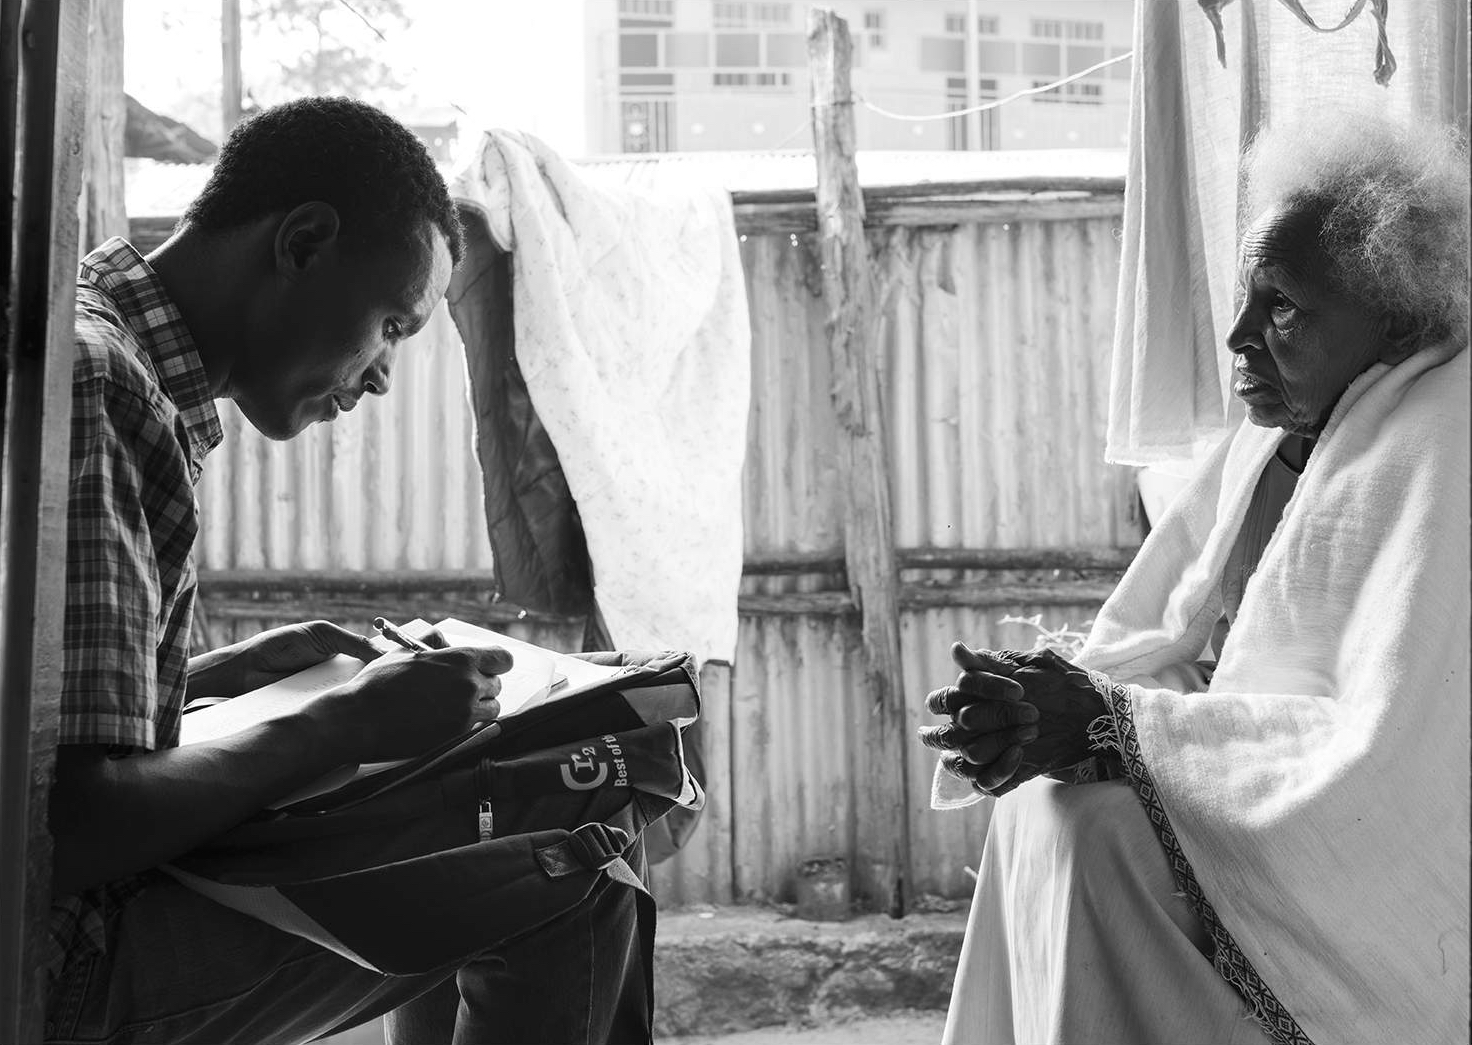
\includegraphics{figures/coverImage.jpg}

\hypertarget{introduction}{%
\chapter*{Introduction}\label{introduction}}
\addcontentsline{toc}{chapter}{Introduction}

Older people (generally defined as people aged sixty years and older)
are a vulnerable group for malnutrition in humanitarian and
developmental contexts. Due to their age they have specific nutritional
needs, such as easily digestible and palatable food adapted to those
with chewing problems, which is dense in nutrients. In famine and
displacement situations where populations are dependent on food
distributions, older people often find the general ration inappropriate
to their tastes and needs, have difficulties accessing the
distributions, or have difficulties transporting rations home. As a
result, older people can become malnourished and in need of specifically
targeted food interventions. In times of drought or food scarcity, older
people tend to reduce their food intake in order to share or give up
their ration to younger members of their families. They are then at risk
of malnutrition.

Despite these potential vulnerabilities in humanitarian situations,
older people are rarely identified as a group in need of specific
nutritional or food assistance. Surveys and assessments almost always
focus on children, and sometimes on pregnant and lactating women.
Humanitarian workers argue that assessing the nutritional status and
needs of older people is both costly and complicated. As a consequence,
the nutritional status and needs of older people in crisis go
unidentified and unaddressed.

HelpAge International, VALID International, and Brixton Health, with
financial assistance from the Humanitarian Innovation Fund (HIF), have
developed a Rapid Assessment Method for Older People (RAM-OP) that
provides accurate and reliable estimates of the needs of older people.
The method uses simple procedures, in a short time frame (i.e.~about two
weeks including training, data collection, data entry, and data
analysis), and at considerably lower cost than other methods. The RAM-OP
method is based on the following principles:

\begin{itemize}
\item
  Use of a familiar ``household survey'' design employing a two-stage
  cluster sample design optimised to allow the use of a small primary
  sample ( m ≥ 16 clusters) and a small overall ( n ≥ 192) sample.
\item
  Assessment of multiple dimensions of need in older people (including
  prevalence of global, moderate and severe acute malnutrition) using,
  whenever possible, standard and well-tested indicators and question
  sets.
\item
  Data analysis performed using modern computer-intensive methods to
  allow estimates of indicator levels to be made with useful precision
  using a small sample size.
\end{itemize}

The following tools are currently available under the General Public
Licence / Free Documentation License, meaning that you are free to copy
and adapt these tools:

\begin{itemize}
\item
  an English language manual / guidebook
\item
  a questionnaire (available in English and French)
\item
  data entry and data checking software (available in English and
  French)
\item
  data analysis software.
\end{itemize}

We believe that the availability of a rapid, low-cost, and user-friendly
method will encourage governments, UN agencies, as well as international
and local non-governmental organisations to actively assess the
situation of older people in humanitarian contexts, and implement,
monitor, and evaluate relevant and timely responses to address their
needs.

\hypertarget{sampling}{%
\chapter{Sampling}\label{sampling}}

\hypertarget{the-ram-op-sample}{%
\section{The RAM-OP sample}\label{the-ram-op-sample}}

RAM-OP uses a two-stage sample:

\textbf{First stage sample:} A sample of communities (e.g.~villages or
city-blocks) in the survey area is taken. A sampled community is also
called a primary sampling unit (PSU).

\textbf{Second stage sample:} Domestic dwellings are sampled from within
the communities selected in the first stage sample. All eligible
individuals in the sampled dwelling are included in the sample.

\hypertarget{the-first-stage-sample}{%
\subsection{The first-stage sample}\label{the-first-stage-sample}}

The first stage sample is a systematic spatial sample. Two methods can
be used and both methods take the sample from all parts of the survey
area:

\begin{itemize}
\tightlist
\item
  \textbf{List-based method:} Communities to be sampled are selected
  systematically from a complete list of communities in the survey area.
  This list of communities is sorted by one or more non-overlapping
  spatial factors such as district and subdistricts within districts:
\end{itemize}

\begin{figure}[H]

{\centering 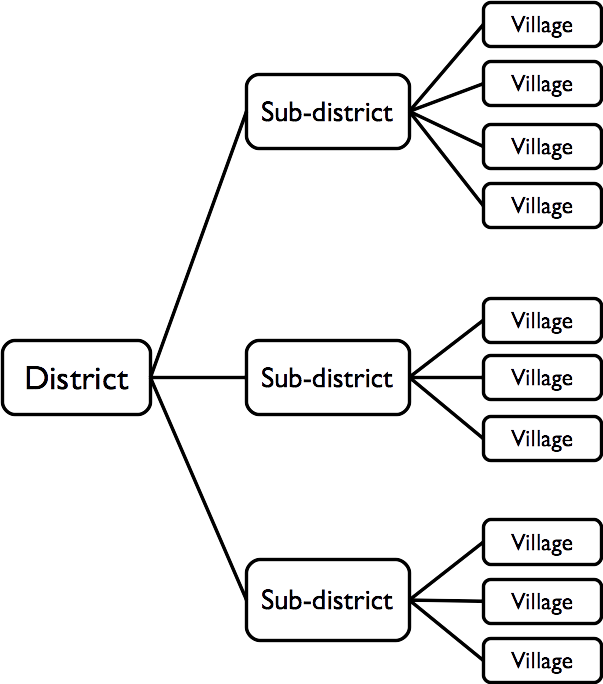
\includegraphics{figures/listSample1} 

}

\caption{Communities listing by district and sub-district}\label{fig:sample1}
\end{figure}

\begin{itemize}
\tightlist
\item
  \textbf{Map-based method:} Communities to be sampled are selected from
  the centres of the squares of a grid drawn over a map. The map must be
  sufficiently well made and of sufficiently large scale to show the
  position of every community in the survey area. This type of sample is
  known as a centric systematic area sample and is often referred to as
  a CSAS sample.
\end{itemize}

\textbf{Note:} \emph{Population proportional sampling} (PPS) is
\textbf{not} used in RAM-OP surveys. Population estimates for all
communities are \textbf{not} required for sampling purposes. Population
estimates are required only for the selected communities. These are used
during data analysis in order to weight results by population size. If
this information is not available before the survey, it can be collected
during the survey.

\hypertarget{the-second-stage-sample}{%
\subsection{The second stage sample}\label{the-second-stage-sample}}

The second stage within-community sample uses a method called
map-segment-sample. This method takes the within-community sample from
all parts of a sampled community.

\hypertarget{implicit-stratification}{%
\section{Implicit stratification}\label{implicit-stratification}}

Both the first and second stage samples use a form of spatial
stratification:

\begin{itemize}
\item
  The list-based method's first stage systematic spatial sample
  stratifies the sample by non-overlapping spatial factor such as
  districts and subdistricts within districts.
\item
  The map-based (CSAS) method's first stage sample stratifies the sample
  by grid square.
\item
  The map-segment-sample second stage within-community sample stratifies
  the sample by parts of the community being sampled.
\item
  The first and second stage samples also ensure that a reasonably even
  spatial sample is taken from the entire survey area and from each of
  the sampled communities.
\end{itemize}

These sampling procedures provide \emph{implicit stratification} and
tend to spread the sample properly among important sub-groups of the
population such as rural / urban / peri-urban populations,
administrative areas, ethnic sub-populations, religious sub-populations,
and socio-economic groups. This often improves the precision of
estimates made from survey data.

The use of implicit stratification improves the efficiency of a
two-stage cluster sample and allows RAM-OP to use relatively small
sample sizes compared to other methods, such as SMART surveys. The use
of modern computer-intensive data analysis techniques also allows RAM-OP
to make better use of the available sample than is done in other
methods.

\newpage

\hypertarget{ram-op-survey-sample-size}{%
\section{RAM-OP survey sample size}\label{ram-op-survey-sample-size}}

The following shorthand symbols will be used when describing sample
designs:

\begin{align*}
m &= \text{Number of primary sampling units (PSUs).} \\[2pt]
n &= \text{Size of the sample of individuals or households from a PSU.} \\[2pt]
n &= \text{May also mean the overall survey sample size (this meaning will be made clear in the text).} \\[2pt]
N &= \text{Population}
\end{align*}

The overall sample size for a RAM-OP survey is about \(n = 192\)
individual subjects. You should aim to collect an overall sample of at
least \(n = 192\) individuals.

The RAM-OP sample is collected in two stages:

\begin{itemize}
\item
  The first stage sample uses a sample size of about \(m = 16\)
  communities (or PSUs).
\item
  The second stage sample uses a sample size of about \(n = 12\)
  eligible subjects sampled from each of the communities selected for
  inclusion in the first stage sample.
\end{itemize}

The overall sample size from \(m = 16\) communities and \(n = 12\)
eligible subjects is about:

\[\text{overall sample size} ~ \approx ~ m ~ \times ~ n ~ \approx ~ 16 ~ \times ~ 12 ~ \approx ~ 192\]

It is not recommended that fewer than \(m = 16\) communities are
sampled.

Sampling fewer than \(m = 16\) communities will tend to reduce the
precision with which estimates can be made. If you have the resources to
sample more than \(m = 16\) communities then you should do so. A sample
of \(m = 24\) communities and \(n = 8\) eligible subjects, for example,
will tend to yield estimates with better precision than a sample with
\(m = 16\) communities and \(n = 12\) eligible subjects.

Do not be tempted to increase the size of the within-community sample in
order to achieve an overall sample size of \(n = 192\) from fewer than
\(m = 16\) communities. Doing so will tend to reduce the precision with
which estimates are made. It may also be impossible to do this in many
settings.

Here, for example, is a \emph{population pyramid} for a typical
developing country:

\begin{figure}[H]

{\centering 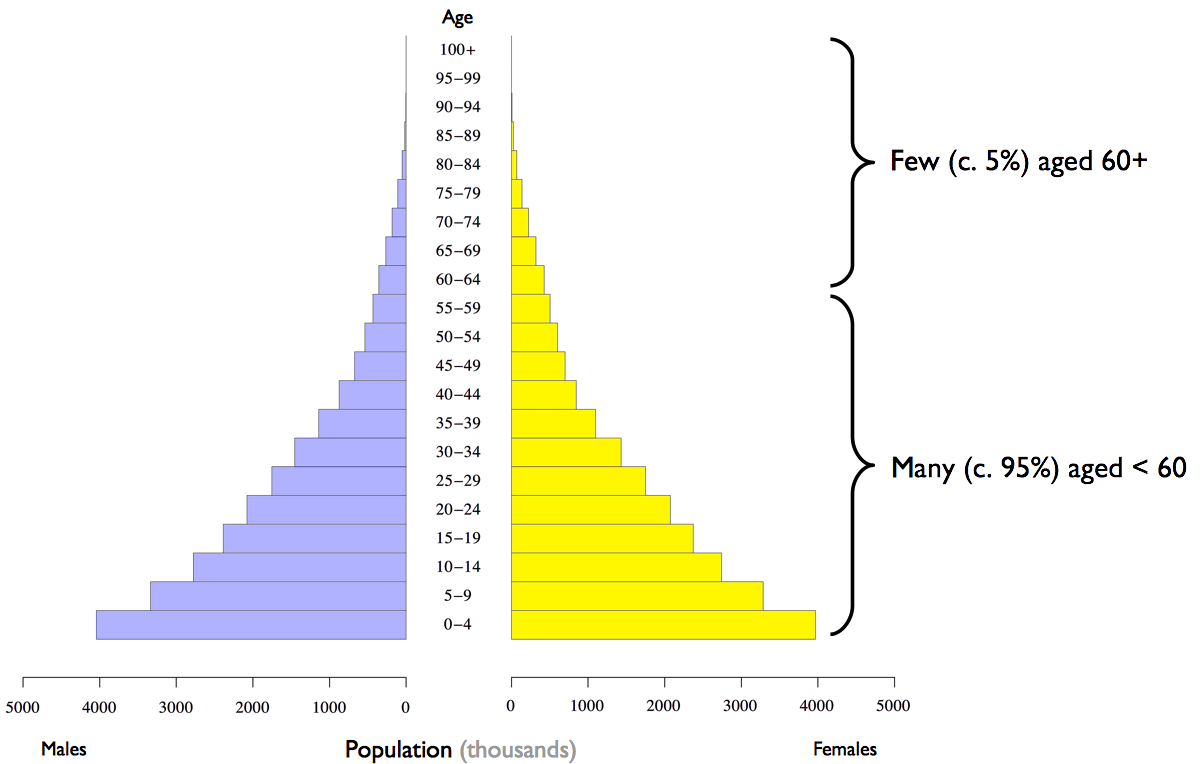
\includegraphics{figures/popPyramid1} 

}

\caption{Population pyramid for a typical developing country}\label{fig:sample2}
\end{figure}

If the average community population is \(N = 300\) then there will be
fewer than 15 people aged 60 years and older in about half of the
selected communities. This is because about half of the selected
communities are likely to have a population below the average
population.

\hypertarget{eligibility}{%
\section{Eligibility}\label{eligibility}}

Older people are usual defined as persons aged 60 years and older (UN
definition). This means your sample will usually be restricted to people
aged 60 years and older.

In some settings different eligibility criteria may apply. This will
likely be the case in settings with very high life-expectancies (usually
middle and high income countries) or very low life-expectancies (usually
low income countries and in emergencies).

In a setting of very high life-expectancy you may want to restrict
eligibility - to persons aged 65 years or older, for example. A local
definition of older people is likely to be available.

In a setting with very low life-expectancy, very few people are aged 60
years or older. For example:

\begin{figure}[H]

{\centering 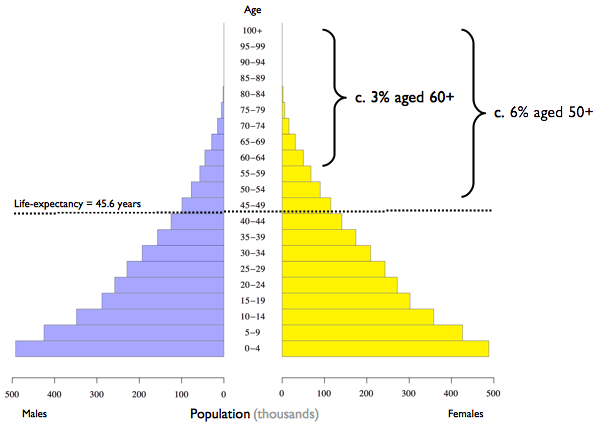
\includegraphics{figures/popPyramid2} 

}

\caption{Population pyramid for a setting with low life-expectancy}\label{fig:sample3}
\end{figure}

It is common in such setting for there to be a local definition of older
people. This will usually be ``persons aged 50 years or older'' or
``persons aged 55 years or older''.

\hypertarget{age-distribution-eligibility-criteria-and-sample-design}{%
\section{Age distribution, eligibility criteria, and sample
design}\label{age-distribution-eligibility-criteria-and-sample-design}}

The age distribution of the population and the survey eligibility
criteria will affect the sample design in terms of the number of
communities that you will need to sample (\(m\)) and the number of older
persons (\(n\)) that can be sampled from each community.

The overall sample size for a RAM-OP sample should be at least
\(n = 192\) usually collected as \(n = 12\) eligible subjects sampled
from \(m = 16\) communities. If older people make up a very small
proportion (i.e.~much less than 5\%) of the total population and / or
the average population of communities is small then you will usually
need to sample more than m = 16 communities in order to get about
\(n = 192\) older people in the overall sample. This is likely to occur
when there are fewer than 20 to 25 older people in a community of
average size.

You can calculate the number of older people that you would expect to be
living in a community of average size using the following formula:

\[n_{\text{aged 60+ in an average village}} ~ = ~ \text{average village population}_{\text{all ages}} ~ \times ~ \frac{\text{percentage of population}_{\text{aged 60+}}}{100}\]

If this is below about 20 people then you should consider how you will
collect the required overall sample size. Three approaches may be used:

\begin{itemize}
\item
  \textbf{Relax the eligibility criteria:} You may decide to define
  older people as ``persons aged 50 years or older'' or ``persons aged
  55 years or older''. This may double the size of the eligible
  population and make the sample easier to collect. This approach is
  only reasonable if life-expectancy is low.
\item
  \textbf{Increase the number of communities that you plan to sample:}
  You may choose to collect your sample as \(n = 7\) eligible subjects
  sampled from \(m = 30\) communities giving an expected overall sample
  size of \(n = 210\). This would be a very good sample. The
  disadvantage of this approach is that survey costs increase with the
  number of communities that are sampled, because a lot of survey time
  and vehicle costs are spent on travelling to and from the selected
  communities.
\item
  \textbf{Take a ``top-up'' sample only when you need to:} The basic
  procedure when a selected community is small and likely to contain
  fewer than \(n = 12\) older people is to collect data on all older
  people in the selected community using a door-to-door census. If the
  within-community sample size is much smaller than the required one
  then a ``top-up'' sample is taken from the nearest neighbouring
  community using the map-segment-sample method (or a door-to-door
  census if this community is also small). The advantage of this
  approach is that travelling time and survey costs are better
  controlled.
\end{itemize}

If the proportion of older people is not very small and / or communities
are large then you should have no problems achieving the overall sample
size.

\hypertarget{practical-sampling}{%
\section{Practical sampling}\label{practical-sampling}}

\hypertarget{the-first-stage-sample---list-based-sampling}{%
\subsection{The first stage sample - list-based
sampling}\label{the-first-stage-sample---list-based-sampling}}

The first stage sample can be drawn from a list of all communities. The
list-based sample is a simple systematic sample taken from a complete
list of communities in the survey area sorted by one or more non-
overlapping spatial factors (such as administrative units or electoral
wards) in the survey area. \emph{Population proportional sampling} (PPS)
is not used since this would concentrate the sample in the larger
communities.

Below is a worked example of how a RAM-OP first stage, list-based sample
can be drawn from a survey area composed of 67 villages.

\textbf{Step 1:} Calculate the \emph{sampling interval} by dividing the
total villages in the survey area (67 villages) with the number of
villages to be drawn from the sample (16 villages).

\[\text{Sampling Interval} ~ = ~ \left \lfloor ~ \frac{N_{\text{villages}}}{N_{\text{sample}}} ~ \right \rfloor ~ = ~ \left \lfloor ~ \frac{67}{16} ~ \right \rfloor ~ \approx ~ \left \lfloor ~ 4.19 ~ \right \rfloor ~ \approx ~ 4\]

The \emph{sampling interval} needs to be a whole number. Remember to
\textbf{always} \emph{round down} when calculating the \emph{sampling
interval} to the nearest whole number.

\textbf{Step 2:} Choose a \emph{random starting point} between 1 and
\emph{sampling interval}. In this example, this would be a random number
\textbf{between 1 and 4}.

A random number can be selected through simple lottery (i.e., draw from
a lot of 4 numbered from 1 to 4). A standard spreadsheet software can
also be used to draw the random number using the \texttt{RANDBETWEEN}
function as follows:

~

\begin{Shaded}
\begin{Highlighting}[]
\KeywordTok{RANDBETWEEN}\NormalTok{(}\DecValTok{1}\NormalTok{, }\DecValTok{4}\NormalTok{)}
\end{Highlighting}
\end{Shaded}

~

\textbf{Step 3:} Using the \emph{random starting point} and the
\emph{sampling interval}, select the sampling villages from a list of
all villages organised/sorted by a \textbf{non-overalapping} spatial
factor such as district or sub-district.

\newpage

\begin{figure}[H]

{\centering 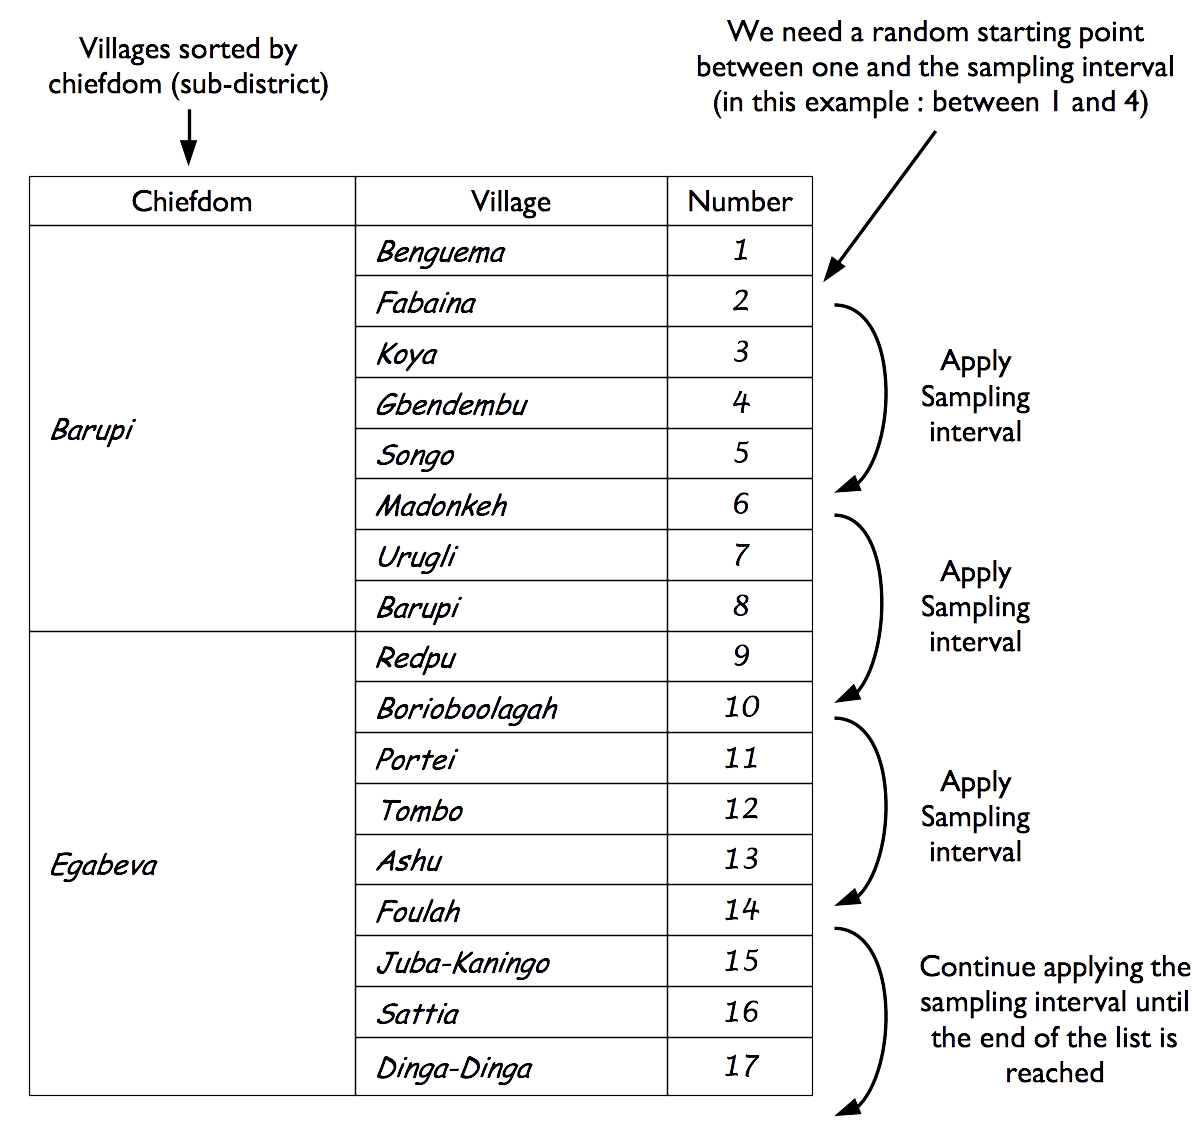
\includegraphics{figures/listSample2} 

}

\caption{Selection of sampling villages using lists}\label{fig:sample4}
\end{figure}

\newpage

\hypertarget{the-first-stage-sample---map-based-sampling}{%
\subsection{The first stage sample - map-based
sampling}\label{the-first-stage-sample---map-based-sampling}}

An alternative approach to list-based sampling is to use map-based
sampling. The map-based (CSAS) sample selects communities from the
centre of squares of a grid drawn over a map. The map must be
sufficiently well made and of sufficiently large scale to show the
position of \textbf{all} communities in the survey area.

A square grid is drawn over the map. The size of the grid squares should
be small enough so that the number of squares covering the survey area
is the same as (or very similar to) the number of communities that you
plan to sample. You may need to experiment with different grid sizes to
achieve this. Figure \ref{fig:sample6} shows an example map and grid
with \(m = 16\) grid squares.

The sample is drawn by selecting the community that is located closest
to the centre of each grid square:

\begin{figure}[H]

{\centering 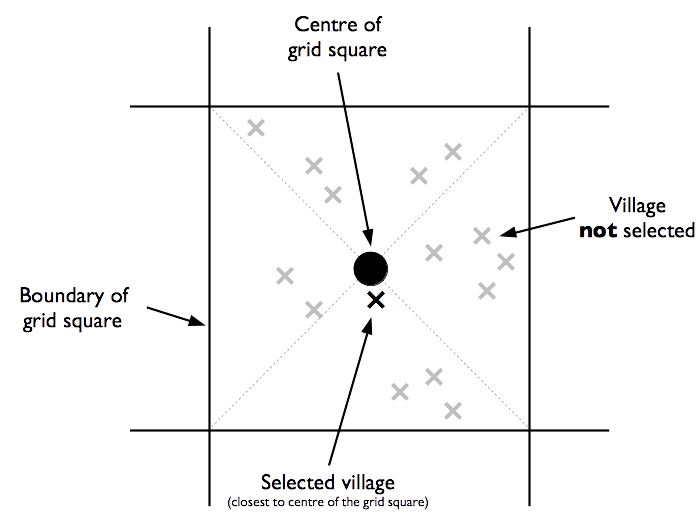
\includegraphics{figures/mapSample1} 

}

\caption{Selection of sampling villages using maps}\label{fig:sample5}
\end{figure}

If two or more villages are located the same distance from the centre of
a grid square then a single village is picked at random, by tossing a
coin for example.

Figure \ref{fig:sample7} shows the sample selected by this process for
the area shown in Figure \ref{fig:sample6}.

\begin{figure}[H]

{\centering 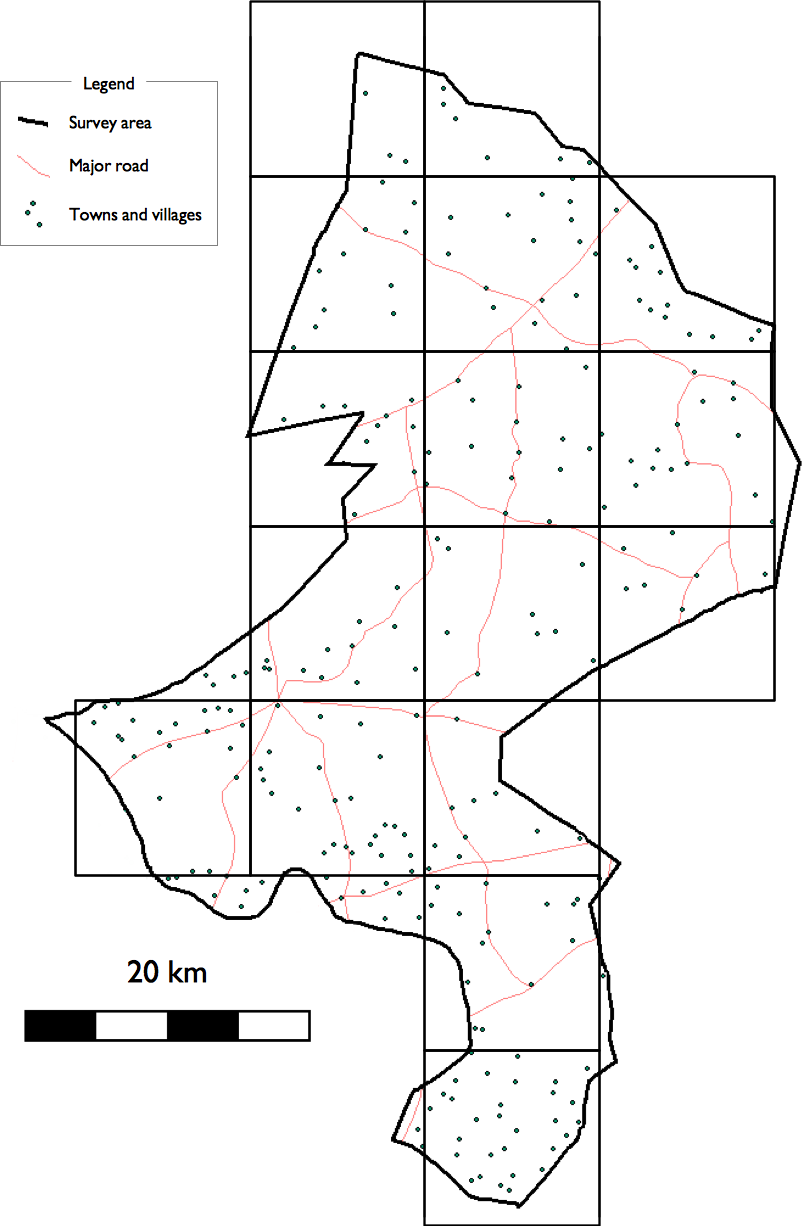
\includegraphics{figures/mapSample2} 

}

\caption{Drawing a square grid over the map}\label{fig:sample6}
\end{figure}

\begin{figure}[H]

{\centering 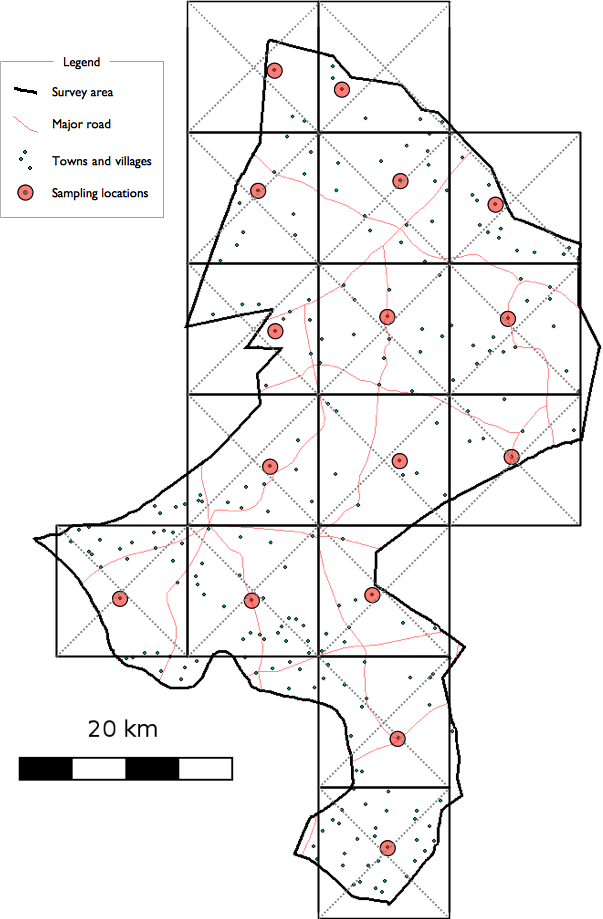
\includegraphics{figures/mapSample3} 

}

\caption{Drawing the first-stage CSAS sample}\label{fig:sample7}
\end{figure}

Both the list-based and the map-based (CSAS) sampling methods spread the
sample of communities evenly across the entire survey area. Each
community has an equal chance of being included in the sample.
Population proportional sampling (PPS) is not used since this would
concentrate the sample in the larger communities.

The same method can be used when sampling in urban contexts. Figure
\ref{fig:sample8} shows a sample drawn from a list of census enumeration
areas sorted by administrative district. Figure \ref{fig:sample9} shows
a sample drawn using the map- based (CSAS) method. In both cases the
primary sampling units (PSUs) are census enumeration areas.

\begin{figure}[H]

{\centering 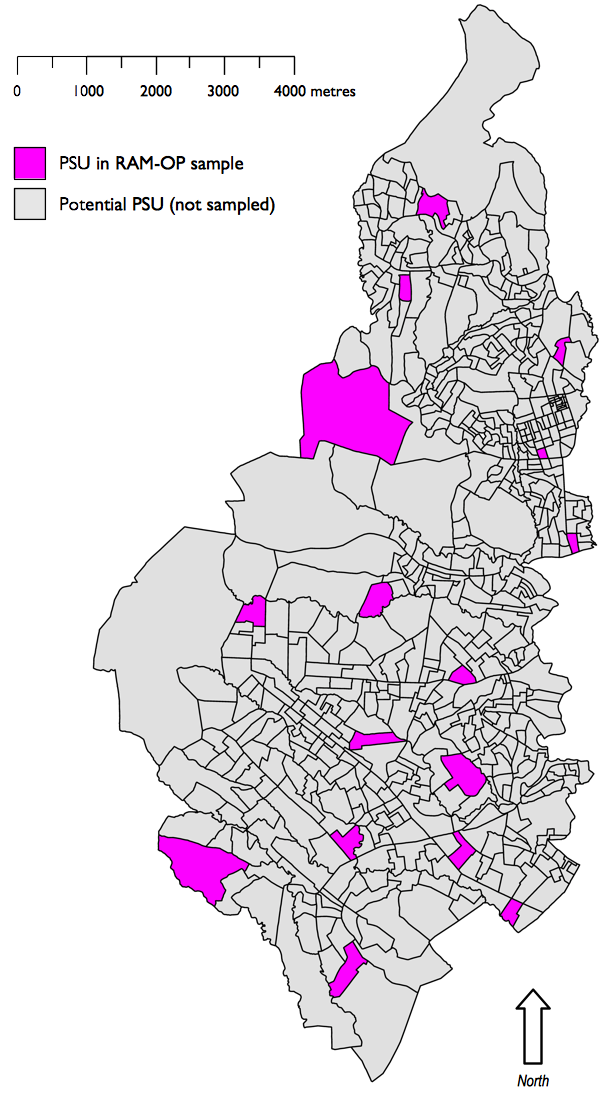
\includegraphics{figures/mapSample4} 

}

\caption{Example of an urban sample (list-based)}\label{fig:sample8}
\end{figure}

\begin{figure}[H]

{\centering 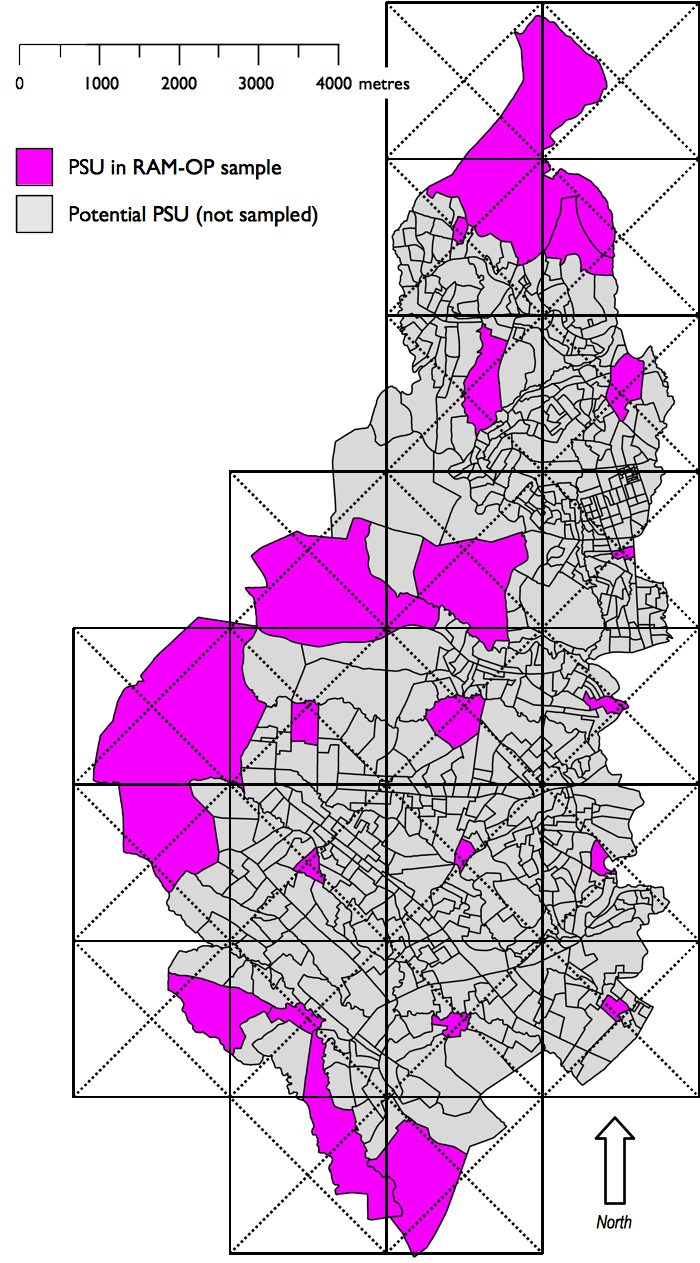
\includegraphics{figures/mapSample5} 

}

\caption{Example of an urban sample (map-based)}\label{fig:sample9}
\end{figure}

\textbf{Note:} In this example twenty-one (21) blocks have been
selected. It can be difficult to achieve exactly the number of blocks
that you need when using this type of sample. It is best to select more
rather than fewer blocks than you need Here we would take our sample as
\(n = 10\) individuals from \(m = 21\) blocks (overall \(n = 210\)).

\hypertarget{the-second-stage-within-community-sample}{%
\subsection{The second stage (within-community)
sample}\label{the-second-stage-within-community-sample}}

The second stage (within-community) sample uses a map-segment-sample
approach:

\textbf{Map:} Make a rough map of the community to be sampled. It is
helpful to think of communities as being made of ribbons (i.e.~lines of
dwellings located along roads, tracks, or rivers) and clusters of
dwellings.

Here is an example of a ribbon of dwellings:

\begin{figure}[H]

{\centering 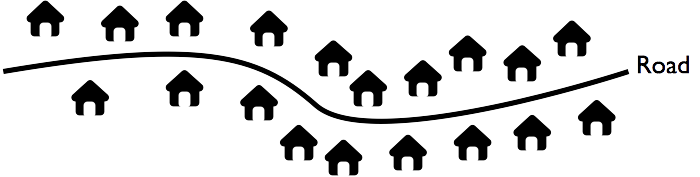
\includegraphics{figures/stage2sample1} 

}

\caption{Example of a ribbon of dwellings}\label{fig:sample10}
\end{figure}

Here is an example of a cluster of dwellings:

\begin{figure}[H]

{\centering 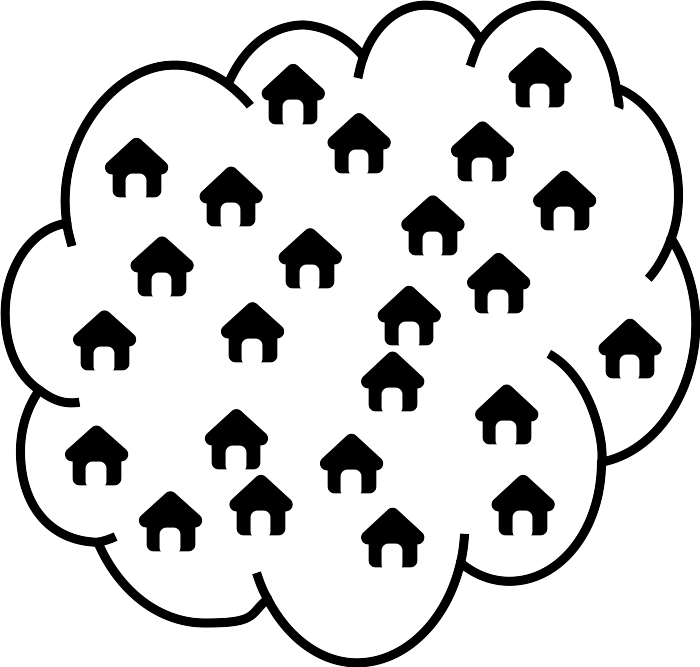
\includegraphics{figures/stage2sample2} 

}

\caption{Example of a cluster of dwellings}\label{fig:sample11}
\end{figure}

\textbf{Segment:} Divide the community into ribbon and cluster segments
defined by the physical layout of the community being sampled.

\textbf{Sample:} Ribbons and clusters are sampled in different ways:

\begin{itemize}
\tightlist
\item
  \textbf{Ribbons} are sampled using \textbf{systematic sampling}.
\item
  \textbf{Clusters} are sampled using a \textbf{random walk} method.
\end{itemize}

\textbf{Note:} If a small community is selected that is likely to have
fewer than the required number of eligible persons then \textbf{all}
eligible persons in that community are sampled by moving door-to-door.

\hypertarget{mapping-the-community---single-and-multiple-clusters}{%
\subsection{Mapping the community - single and multiple
clusters}\label{mapping-the-community---single-and-multiple-clusters}}

Some communities consist of a single cluster of dwellings:

\begin{figure}[H]

{\centering 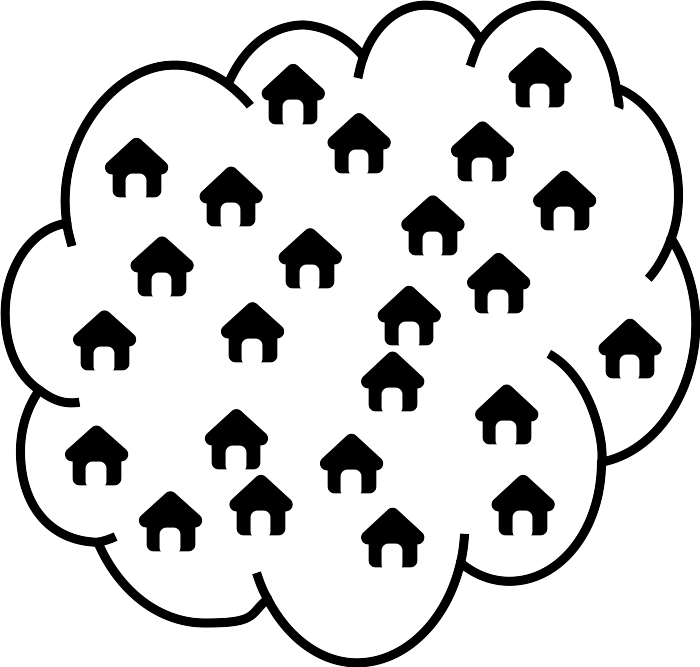
\includegraphics{figures/stage2sample2} 

}

\caption{Example of a cluster of dwellings}\label{fig:sample12}
\end{figure}

or a set of clusters of dwellings:

\begin{figure}[H]

{\centering 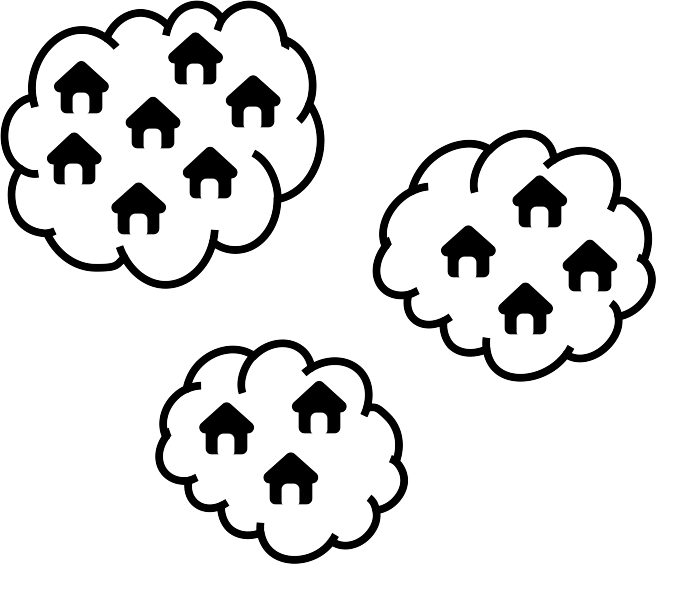
\includegraphics{figures/stage2sample3} 

}

\caption{Example of a set of clusters of dwellings}\label{fig:sample13}
\end{figure}

For communities (or parts of communities) structured in this way we use
a sampling method called the \textbf{random walk}.

\hypertarget{mapping-the-community---ribbon-communities}{%
\subsection{Mapping the community - ribbon
communities}\label{mapping-the-community---ribbon-communities}}

Ribbon communities have dwellings arranged in a line:

\begin{figure}[H]

{\centering 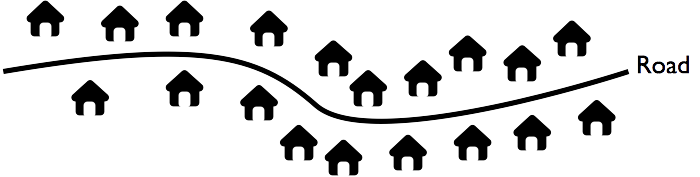
\includegraphics{figures/stage2sample1} 

}

\caption{Dwellings arranged in a line}\label{fig:sample14}
\end{figure}

or in a several lines:

\begin{figure}[H]

{\centering 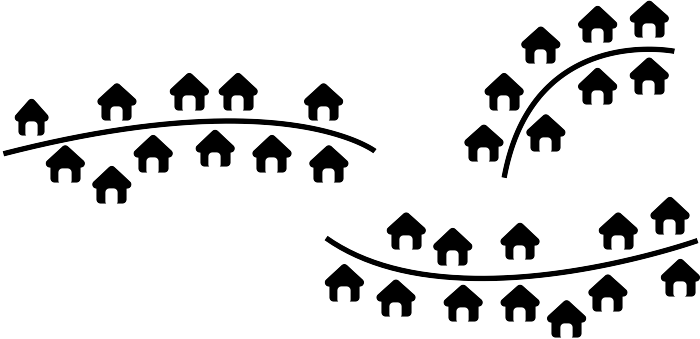
\includegraphics{figures/stage2sample4} 

}

\caption{Dwellings arranged in several lines}\label{fig:sample15}
\end{figure}

For communities (or parts of communities) structured in this way we use
a sampling method called \textbf{systematic sampling}.

\hypertarget{mapping-the-community---mixed-communities}{%
\subsection{Mapping the community - mixed
communities}\label{mapping-the-community---mixed-communities}}

Some communities are a mixture of clusters and ribbons:

\begin{figure}[H]

{\centering 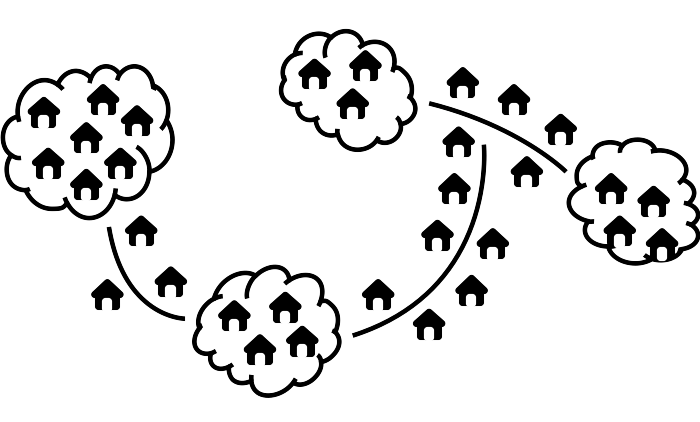
\includegraphics{figures/stage2sample5} 

}

\caption{Mixture of clusters and ribbons}\label{fig:sample16}
\end{figure}

For mixed communities we use a mixture of the \textbf{random walk}
method (in the clusters) and \textbf{systematic sampling} (along the
ribbons).

\textbf{Segmentation} involves dividing a community into several parts
and taking part of the within-community sample from each
\textbf{segment}. With simple communities, segmentation is not required
and we take a single sample from the entire community using the
appropriate sampling method.

\hypertarget{segmentation}{%
\subsection{Segmentation}\label{segmentation}}

For more complicated communities we divide the community into several
parts or segments, such as a community made up of several clusters:

\begin{figure}[H]

{\centering 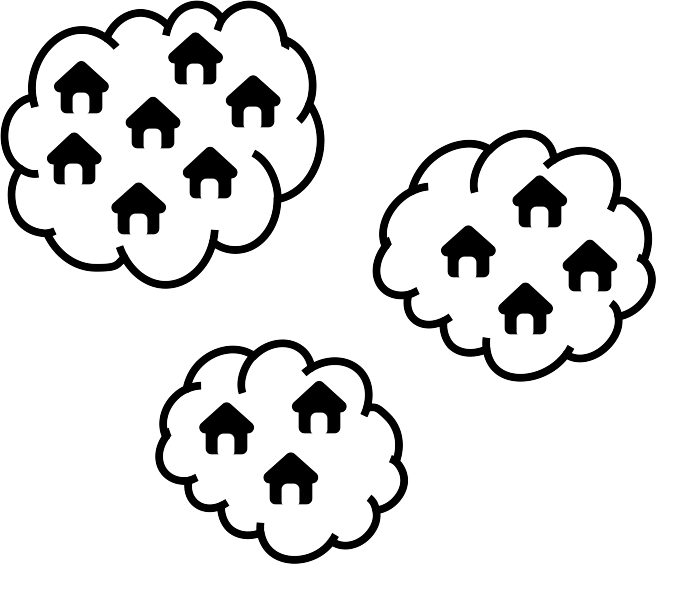
\includegraphics{figures/stage2sample3} 

}

\caption{Example of a set of clusters of dwellings}\label{fig:sample17}
\end{figure}

or a community made up of several ribbons:

\begin{figure}[H]

{\centering 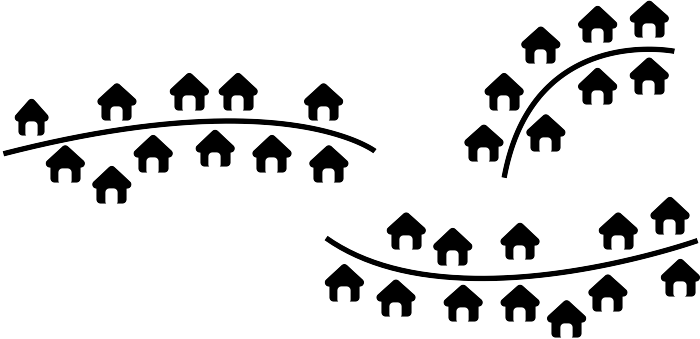
\includegraphics{figures/stage2sample4} 

}

\caption{Dwellings arranged in several lines}\label{fig:sample18}
\end{figure}

or a mixed community:

\begin{figure}[H]

{\centering 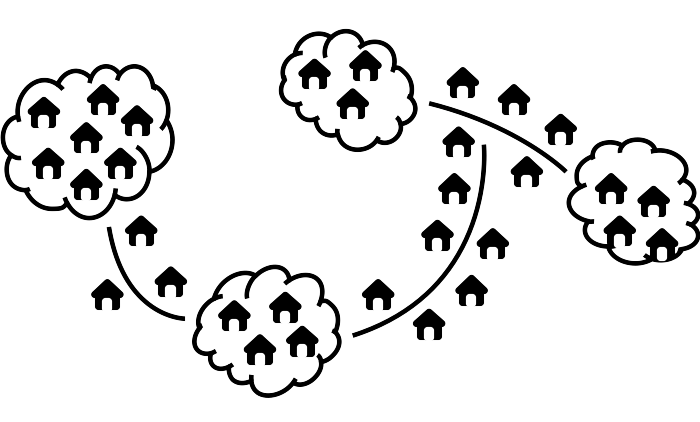
\includegraphics{figures/stage2sample5} 

}

\caption{Mixture of clusters and ribbons}\label{fig:sample19}
\end{figure}

We take a small sample from each segment using the appropriate sampling
method.

For example, with a community made up of three segments:

\begin{figure}[H]

{\centering 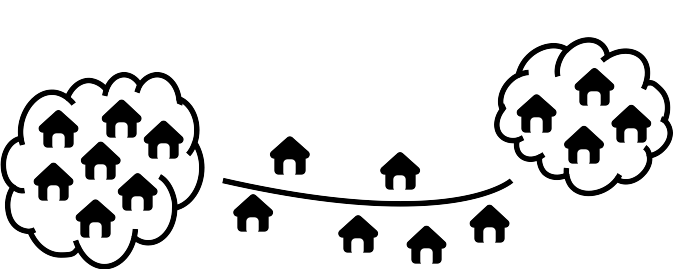
\includegraphics{figures/stage2sample6} 

}

\caption{Community made up of three segments}\label{fig:sample20}
\end{figure}

we would take one third of the overall sample from each segment.

If the within-community sample size is twelve eligible subjects. we
would sample four eligible subjects from each segment (i.e.
\(12 / 3 = 4\)).

Dividing the sample up in this way means that we will sample from every
part of the community rather than just one part of the community.

When taking the sample we use the random walk method to take part of the
sample from clusters and the systematic sampling method to take part of
the sample from ribbons.

Segments should be either ribbons or clusters but should \textbf{never}
contain both a ribbon and a cluster. This is because clusters and
ribbons are sampled in different ways.

A dwelling can only belong to one segment. Segments should \textbf{not}
overlap.

\hypertarget{sample-dwellings}{%
\subsection{Sample dwellings}\label{sample-dwellings}}

\textbf{All} segments should be sampled.

If, for example, there are five segments in a community:

\begin{figure}[H]

{\centering 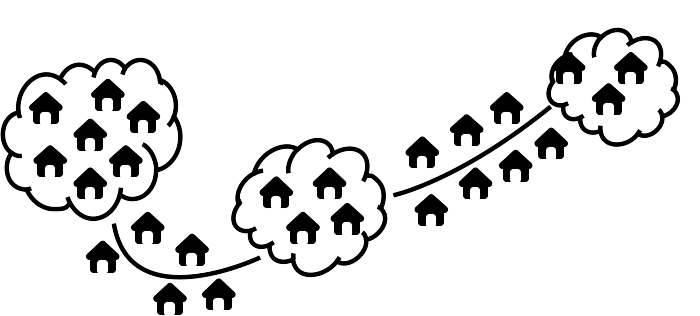
\includegraphics{figures/stage2sample7} 

}

\caption{Community made up of five segments}\label{fig:sample21}
\end{figure}

and the within-community sample size is twelve eligible subjects, then
you would plan to sample two eligible subjects from each segment (i.e.
\(12 / 5 = 2.4\) \textbf{rounded down} to two) and, if necessary, return
to the \textbf{largest} segment to complete the sample.

\textbf{All} segments should be sampled, even if this means that you
take a larger sample than you expected to.

Remember that different types of segment are sampled in different ways:

\begin{itemize}
\item
  Dwellings in \textbf{cluster segments} are sampled using a method
  called the \textbf{random walk}. This involves sampling houses by
  walking in random directions within the cluster.
\item
  Dwellings in \textbf{ribbon segments} are sampled using a method
  called \textbf{systematic sampling}. This involves sampling houses at
  regular intervals along the ribbon.
\end{itemize}

We will look at each of these sampling methods in turn.

\hypertarget{random-walk-sampling}{%
\subsection{Random walk sampling}\label{random-walk-sampling}}

The \textbf{random walk} method is used to sample dwellings in
\textbf{cluster segments}. Sampling proceeds as follows:

\begin{enumerate}
\def\labelenumi{\arabic{enumi}.}
\item
  Move to the approximate centre of the cluster.
\item
  Select a \textbf{random direction} by spinning a bottle on the ground.
  The neck indicates the \textbf{sampling direction}. This is the
  direction you should walk in order to sample a dwelling. Walk in the
  sampling direction counting the dwellings that you pass. Sample the
  third \textbf{dwelling}. If there are no eligible persons in the
  selected dwelling then sample the \textbf{nearest} dwelling with an
  eligible person. Sample \textbf{all} eligible persons in the selected
  dwelling.
\item
  Apply the survey questionnaire for \textbf{all} eligible persons in
  the selected dwelling.
\item
  Select the next dwelling to sample by spinning a bottle and walking in
  the indicated direction. Count the dwellings you pass. Sample the
  \textbf{third} dwelling. If there are no eligible persons in the
  selected dwelling then sample the \textbf{nearest} dwelling with an
  eligible person. Sample all eligible persons in the selected dwelling.
  If you reach the edge of the cluster segment then return to the centre
  of the cluster and repeat step (2) above. Remember to keep count of
  the number of eligible persons sampled from the segment.
\item
  Stop sampling in the segment when you have sampled the required number
  of eligible persons from the segment. Since you sample \textbf{all}
  eligible persons in a selected dwelling, you may sample a few more
  eligible persons than expected. This is OK. Always sample \textbf{all}
  eligible persons in a selected dwelling.
\end{enumerate}

If, when you have sampled all segments, you have not sampled twelve
eligible persons, you should return to the \textbf{largest} segment to
finish sampling using the appropriate sampling method.

The random walk method is illustrated in Figure \ref{fig:sample22}.

\begin{figure}[H]

{\centering 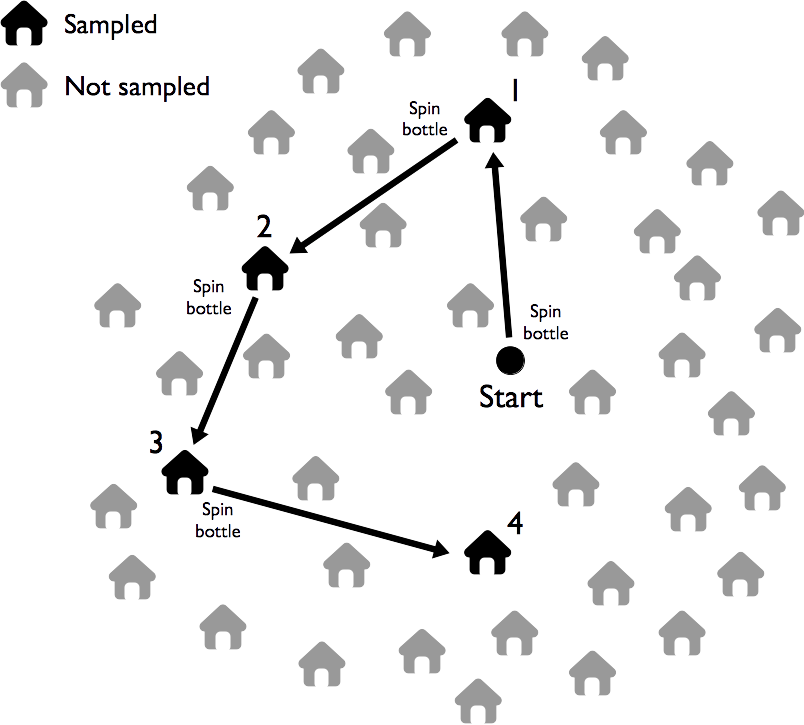
\includegraphics{figures/stage2sample8} 

}

\caption{Random walk sampling in a cluster segment}\label{fig:sample22}
\end{figure}

\hypertarget{systematic-sampling}{%
\subsection{Systematic sampling}\label{systematic-sampling}}

The \textbf{systematic sampling} method is used to sample houses in
\textbf{ribbon segments}.

Sampling proceeds as follows:

\begin{enumerate}
\def\labelenumi{\arabic{enumi}.}
\item
  Move to one end of the ribbon segment.
\item
  Walk to the other end of the segment counting the houses that you
  pass.
\item
  Calculate the \textbf{step size} by dividing the number of dwellings
  in the segment by the required sample size for the segment. Use the
  \textbf{whole number} part of the result only. Do \textbf{not} round
  up.
\item
  Pick a random number between one and the step size. This is your
  \textbf{starting point}. Select the first dwelling to sample by
  walking along the segment counting the dwellings that you pass and
  sample the dwelling indicated by the \textbf{starting point}. If there
  are no eligible persons in the selected dwelling then sample the
  \textbf{nearest} dwelling in any direction with an eligible person.
  Sample \textbf{all} eligible persons in the selected dwelling.
\item
  Select the next dwelling to sample by walking along the segment. Count
  the dwellings that you pass. Sample the dwelling indicated by the
  \textbf{step size}. If there are no eligible persons in the selected
  dwelling then sample the \textbf{nearest} dwelling in any direction
  with an eligible person. Sample \textbf{all} eligible persons in the
  selected dwelling.
\item
  Stop sampling in the segment when you reach the end of the ribbon
  segment. This may mean that you sample extra eligible persons. This is
  OK. Do \textbf{not} stop sampling from a ribbon until you reach the
  end of the ribbon.
\end{enumerate}

If, when you have sampled all segments, you have not sampled twelve
eligible persons, you should return to the \textbf{largest} segment to
finish sampling using the appropriate sampling method.

The systematic sampling method is illustrated in Figure
\ref{fig:sample23}.

\begin{figure}[H]

{\centering 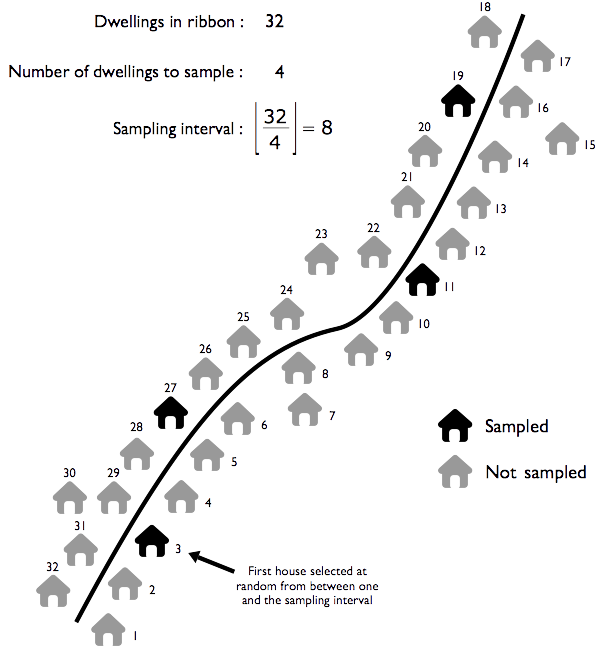
\includegraphics{figures/stage2sample9} 

}

\caption{Systematic sampling in a ribbon segment}\label{fig:sample23}
\end{figure}

\hypertarget{sampling-in-urban-settings}{%
\subsection{Sampling in urban
settings}\label{sampling-in-urban-settings}}

In urban areas the first stage sample is taken by replacing
sub-districts with ``sections'' and communities with city blocks.
Examples of sections may be administrative districts/sub-districts or
electoral wards.

\begin{figure}[H]

{\centering 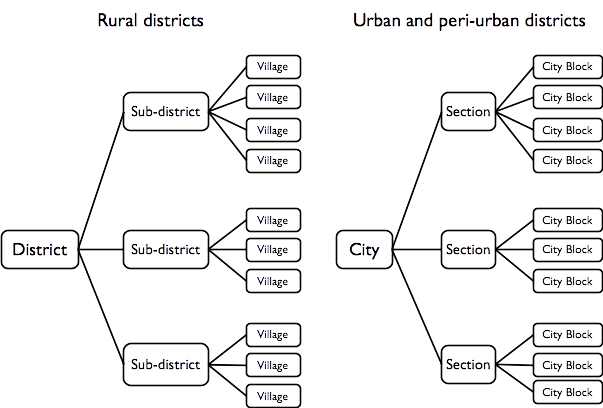
\includegraphics{figures/stage2sample10} 

}

\caption{Administrative divisions in an urban setting}\label{fig:sample24}
\end{figure}

Census enumeration areas (EAs) are usually city blocks. Central
statistics offices can usually provide lists of EAs by ``section'' and
large-scale maps of EAs selected for sampling (See Figure
\ref{fig:sample25} and Figure \ref{fig:sample26}). These maps make it
easy to locate EAs and their boundaries. The sample of EAs can be
decided using list-based or map-based (CSAS) sampling.

In these settings, eligible persons may be sampled by moving from
door-to-door. All dwellings in the selected block are sampled and all
eligible persons in the selected dwellings are sampled. This means that
all eligible persons in a selected block are sampled.

If city blocks are large then a type of systematic sampling may be used.
With this method a rough map of the streets in the block is made and the
number of doorways on each street is counted and copied onto the rough
street map (as shown in Figure \ref{fig:sample27}). The total number of
doorways on all streets is calculated. A step size is calculated by
dividing the total number of doorways on all streets by the number of
dwellings to be sampled. A systematic sample along a route around the
block that includes all streets in the block is taken. Streets can be
sampled in any order. If you find that you have sampled all streets but
have not yet sampled the required number of eligible persons then you
should return to the street with the largest number of houses to collect
the remainder of the sample.

The number of blocks to be sampled will depend on the expected number of
eligible persons in each block. You should aim for an overall sample
size of about \(n = 192\). You should not sample fewer than \(m = 16\)
blocks.

\begin{figure}[H]

{\centering 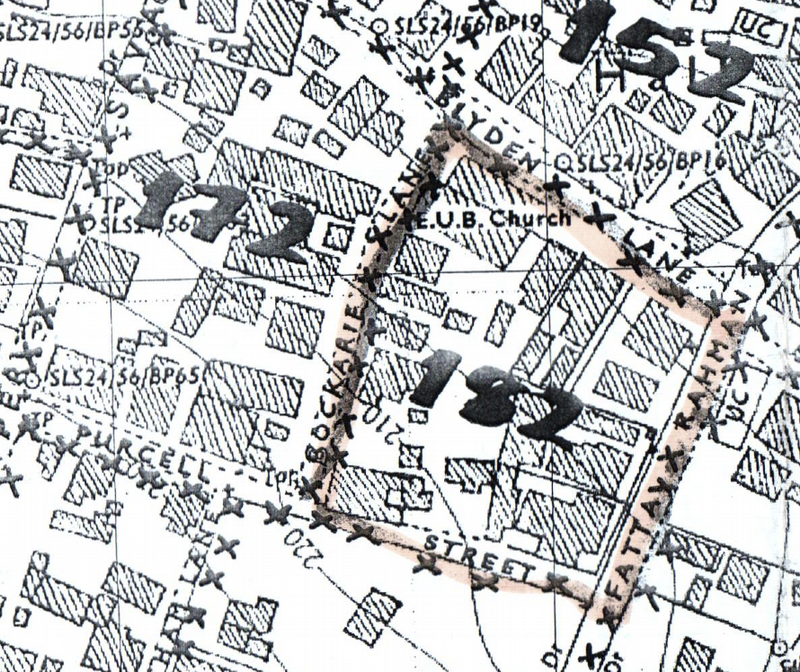
\includegraphics{figures/stage2sample11} 

}

\caption{Enumeration area map for a city block in Freetown, Sierra Leone}\label{fig:sample25}
\end{figure}

\newpage

\begin{figure}[H]

{\centering 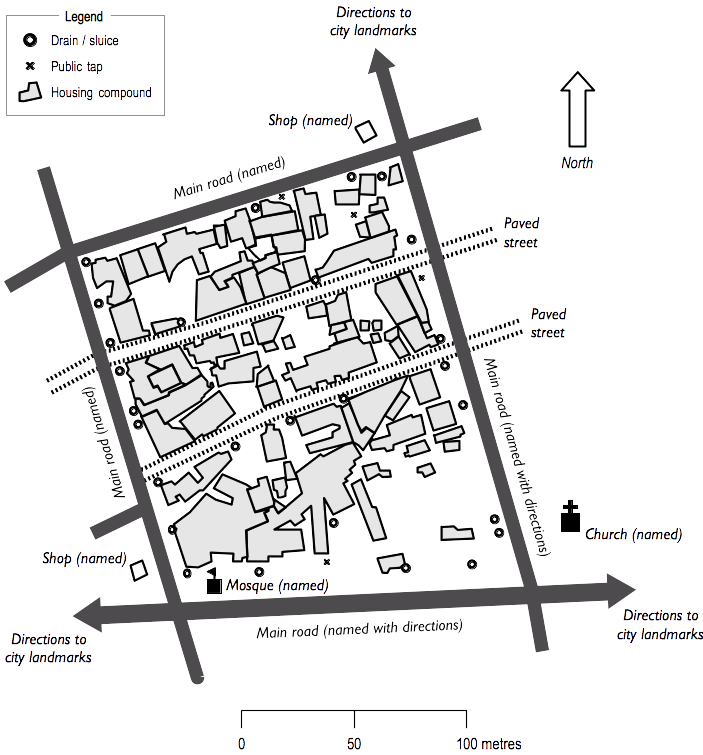
\includegraphics{figures/stage2sample12} 

}

\caption{Enumeration area map for a city block in Addis Ababa, Ethiopia}\label{fig:sample26}
\end{figure}

\begin{figure}[H]

{\centering 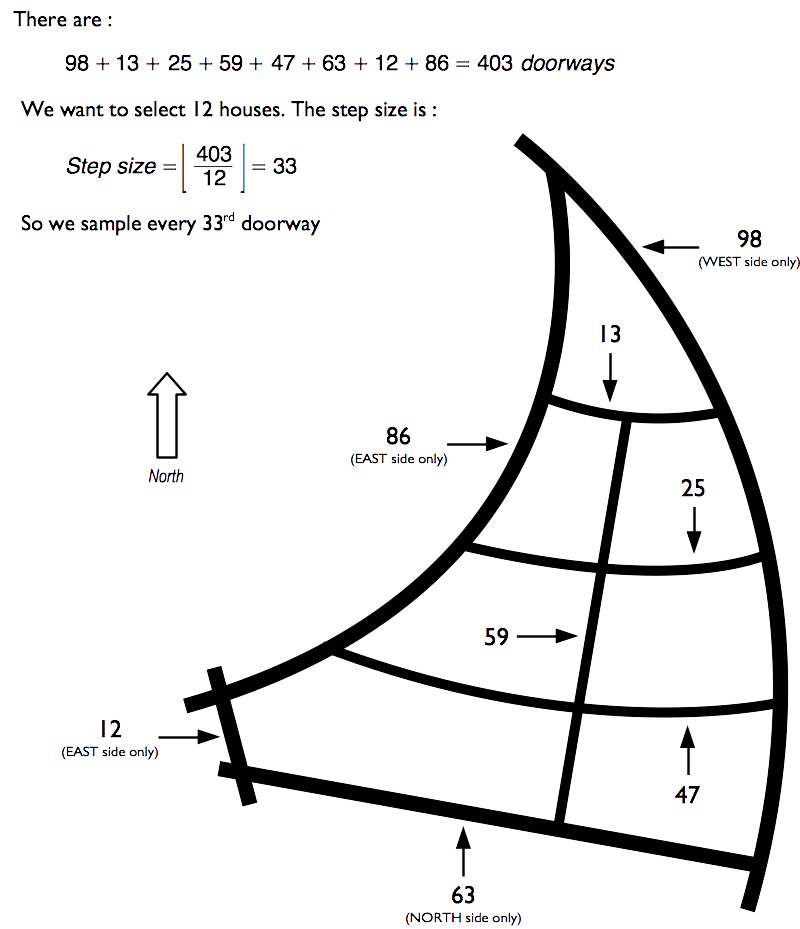
\includegraphics{figures/stage2sample13} 

}

\caption{Systematic sampling in a city block}\label{fig:sample27}
\end{figure}

When useful lists and maps are not available then satellite imagery
available though free services such as Google Earth
(\url{http://earth.google.com}) may be used.

The quality (resolution) of the images available from these services is
variable but is usually good enough to allow you to segment the town
into small areas of approximately equal volume (approximately the same
number of dwellings) in each:

\begin{figure}[H]

{\centering 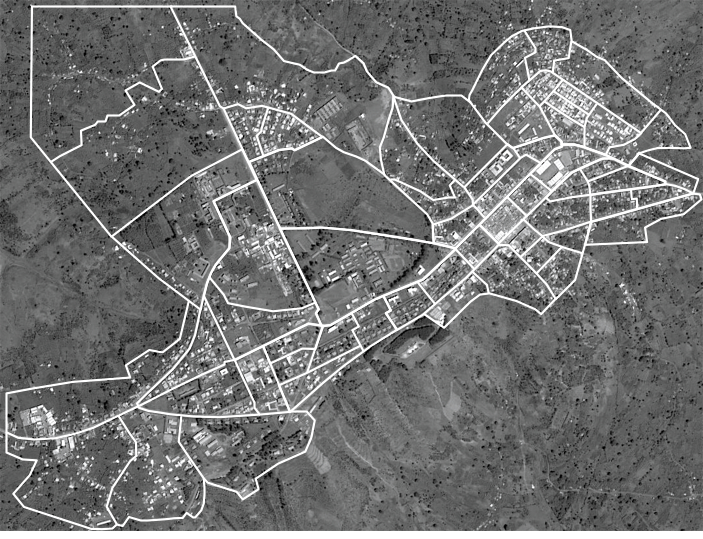
\includegraphics{figures/stage2sample14} 

}

\caption{Segmenting a town into smaller sampling areas}\label{fig:sample28}
\end{figure}

When creating segments using maps or satellite images it is a good idea
to use main roads, rivers, canals, railway lines, public parks, etc as
boundaries. This simplifies the segmentation process and also simplifies
fieldwork by making areas and their boundaries easier to locate and
sample.

The first stage sample can be list-based (such as where each area is
numbered in a systematic north to south and east to west order and a
systematic sample taken) or map-based (CSAS).

Larger scale ``maps'' of blocks to be sampled can also me made using
satellite imagery (see Figure \ref{fig:sample29}).

\newpage

\begin{figure}[H]

{\centering 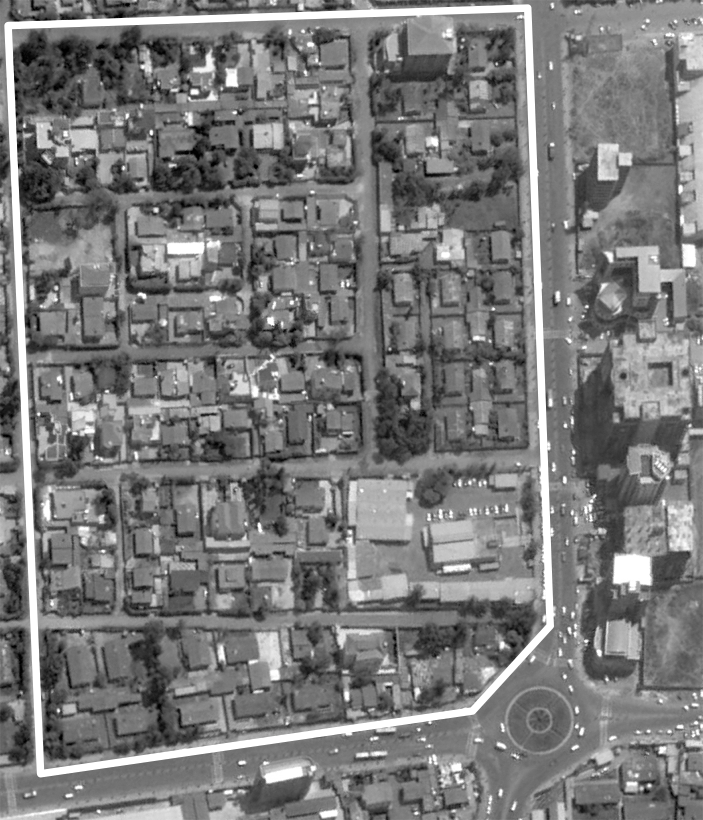
\includegraphics{figures/stage2sample15} 

}

\caption{A large scale “map” of a city block made from satellite imagery}\label{fig:sample29}
\end{figure}

\hypertarget{indicators}{%
\chapter{Indicators}\label{indicators}}

\hypertarget{the-ram-op-indicator-set}{%
\section{The RAM-OP indicator set}\label{the-ram-op-indicator-set}}

RAM-OP surveys collect and report on data for a broad range of
indicators relevant to older people.

These indicators cover the following dimensions:

\begin{itemize}
\tightlist
\item
  Demography and situation
\item
  Food intake
\item
  Severe food insecurity
\item
  Disability
\item
  Activities of daily living
\item
  Mental health and well-being
\item
  Dementia
\item
  Health and health-seeking behaviour
\item
  Sources of income
\item
  Water, sanitation, and hygiene
\item
  Anthropometry and screening coverage
\item
  Visual impairment
\end{itemize}

Data for a small group of miscellaneous indicators are also collected
and reported.

The RAM-OP indicator set has been designed on a modular basis. Each
module is a set of indicators relating to a single dimension from the
list given above and is collected using a dedicated set of questions and
measurements. This means that the RAM-OP questionnaire also consists of
a set of modules.

Whenever possible, RAM-OP uses standard and validated indicators and
question sets.

Indicators are described below, showing the questionnaire components
that are used to collect and record the data required, and flowcharts of
the process used to derive indicators from the collected data. Standard
symbols are used. For example:

\begin{center}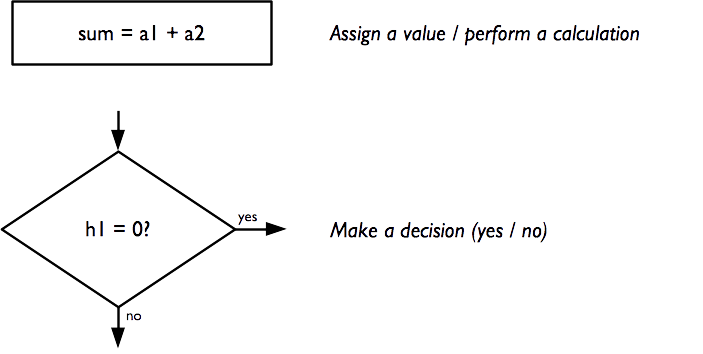
\includegraphics{figures/indicators01} \end{center}

A non-standard symbol is used to show \textbf{recode operations}. A
recode operation shows changes that are made to data so that it can be
used to derive indicators without having to show many decision nodes in
the flowchart. They are also used to specify what should be done with
missing or out-of-range values. For example:

\begin{center}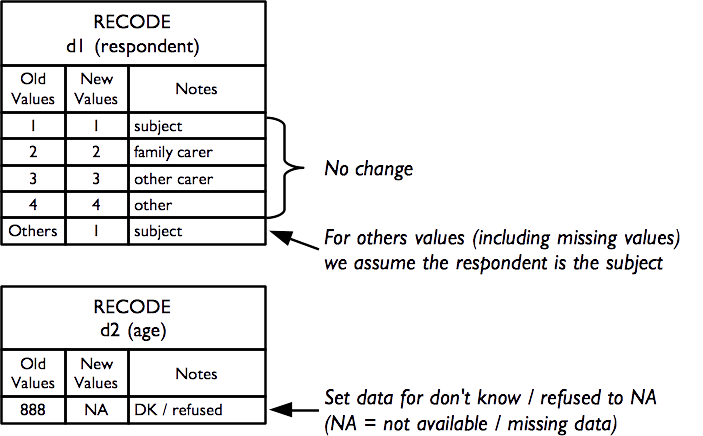
\includegraphics{figures/indicators02} \end{center}

\hypertarget{demography-and-situation}{%
\subsection{Demography and situation}\label{demography-and-situation}}

The demography and situation indicators are used to describe the survey
sample and are derived from this questionnaire component:

\begin{center}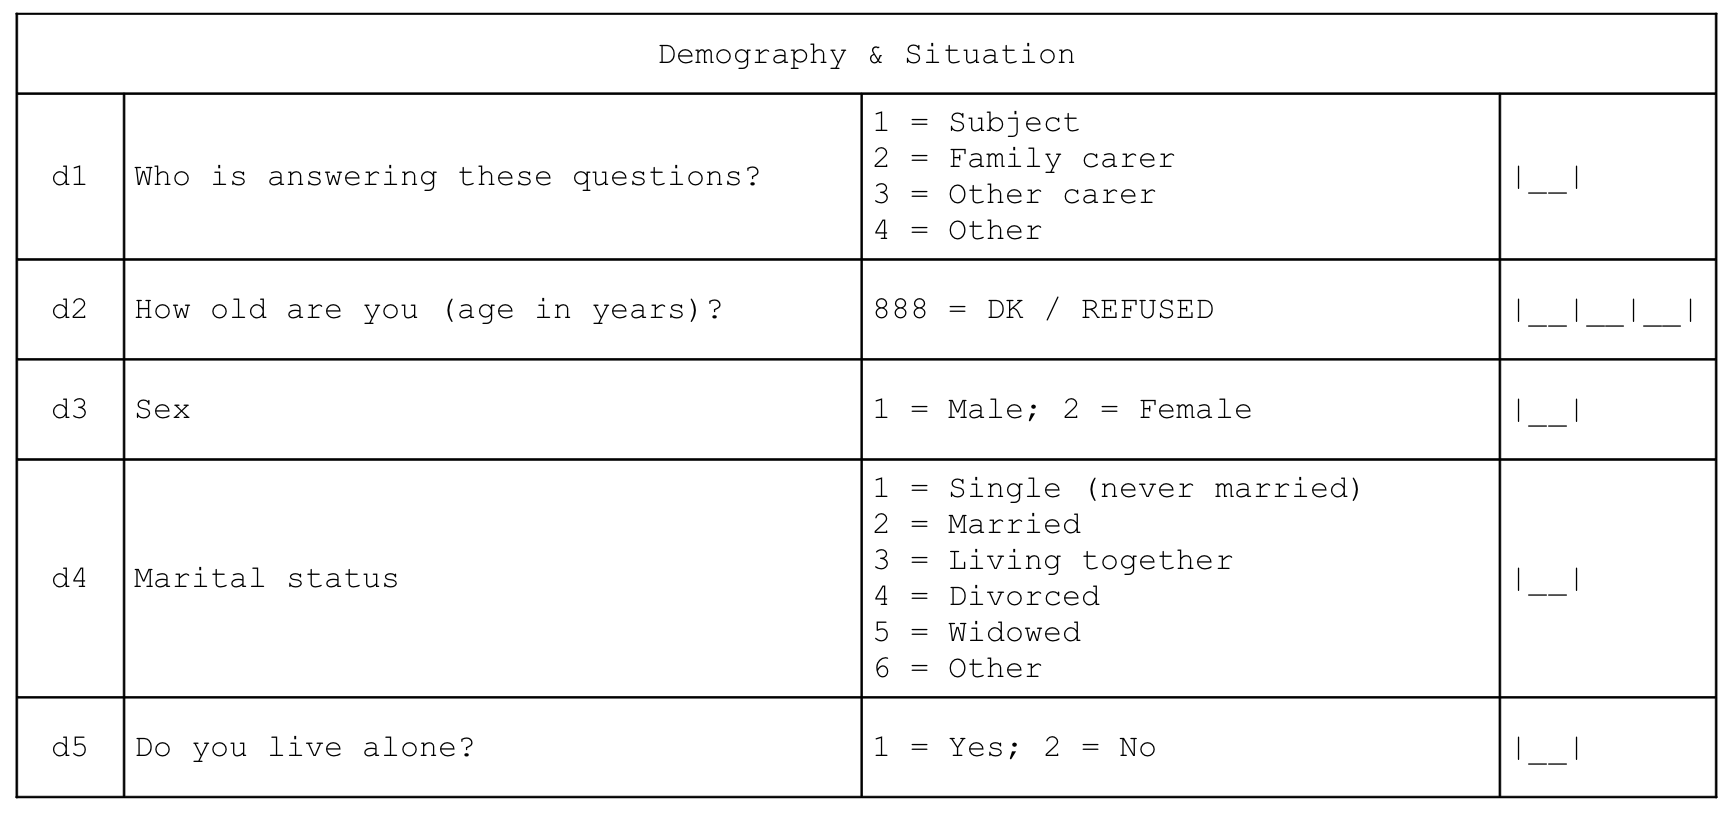
\includegraphics{figures/questionnaire01} \end{center}

\newpage

Each of the questions yields a separate indicator:

\begin{center}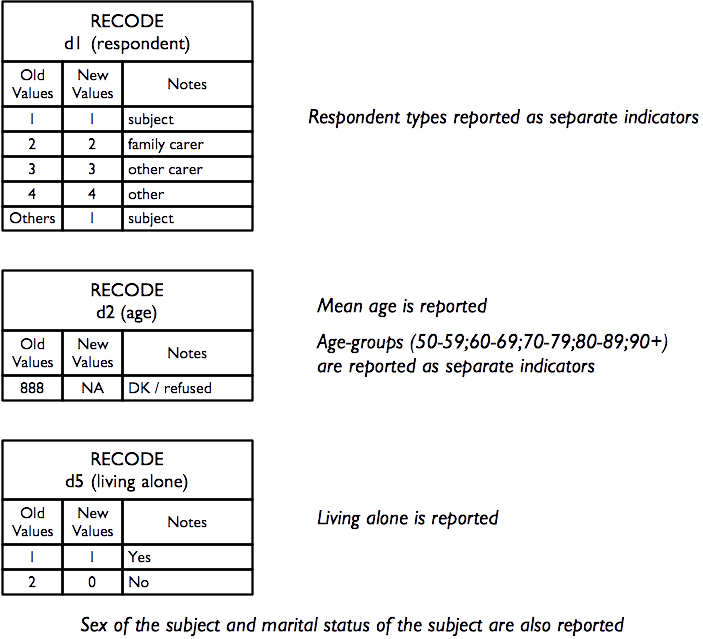
\includegraphics{figures/indicators03} \end{center}

\hypertarget{food-intake}{%
\subsection{Food intake}\label{food-intake}}

Food-intake indicators are derived from this questionnaire component.
This data can be queried to yield a large number of useful indicators.

\newpage

\begin{center}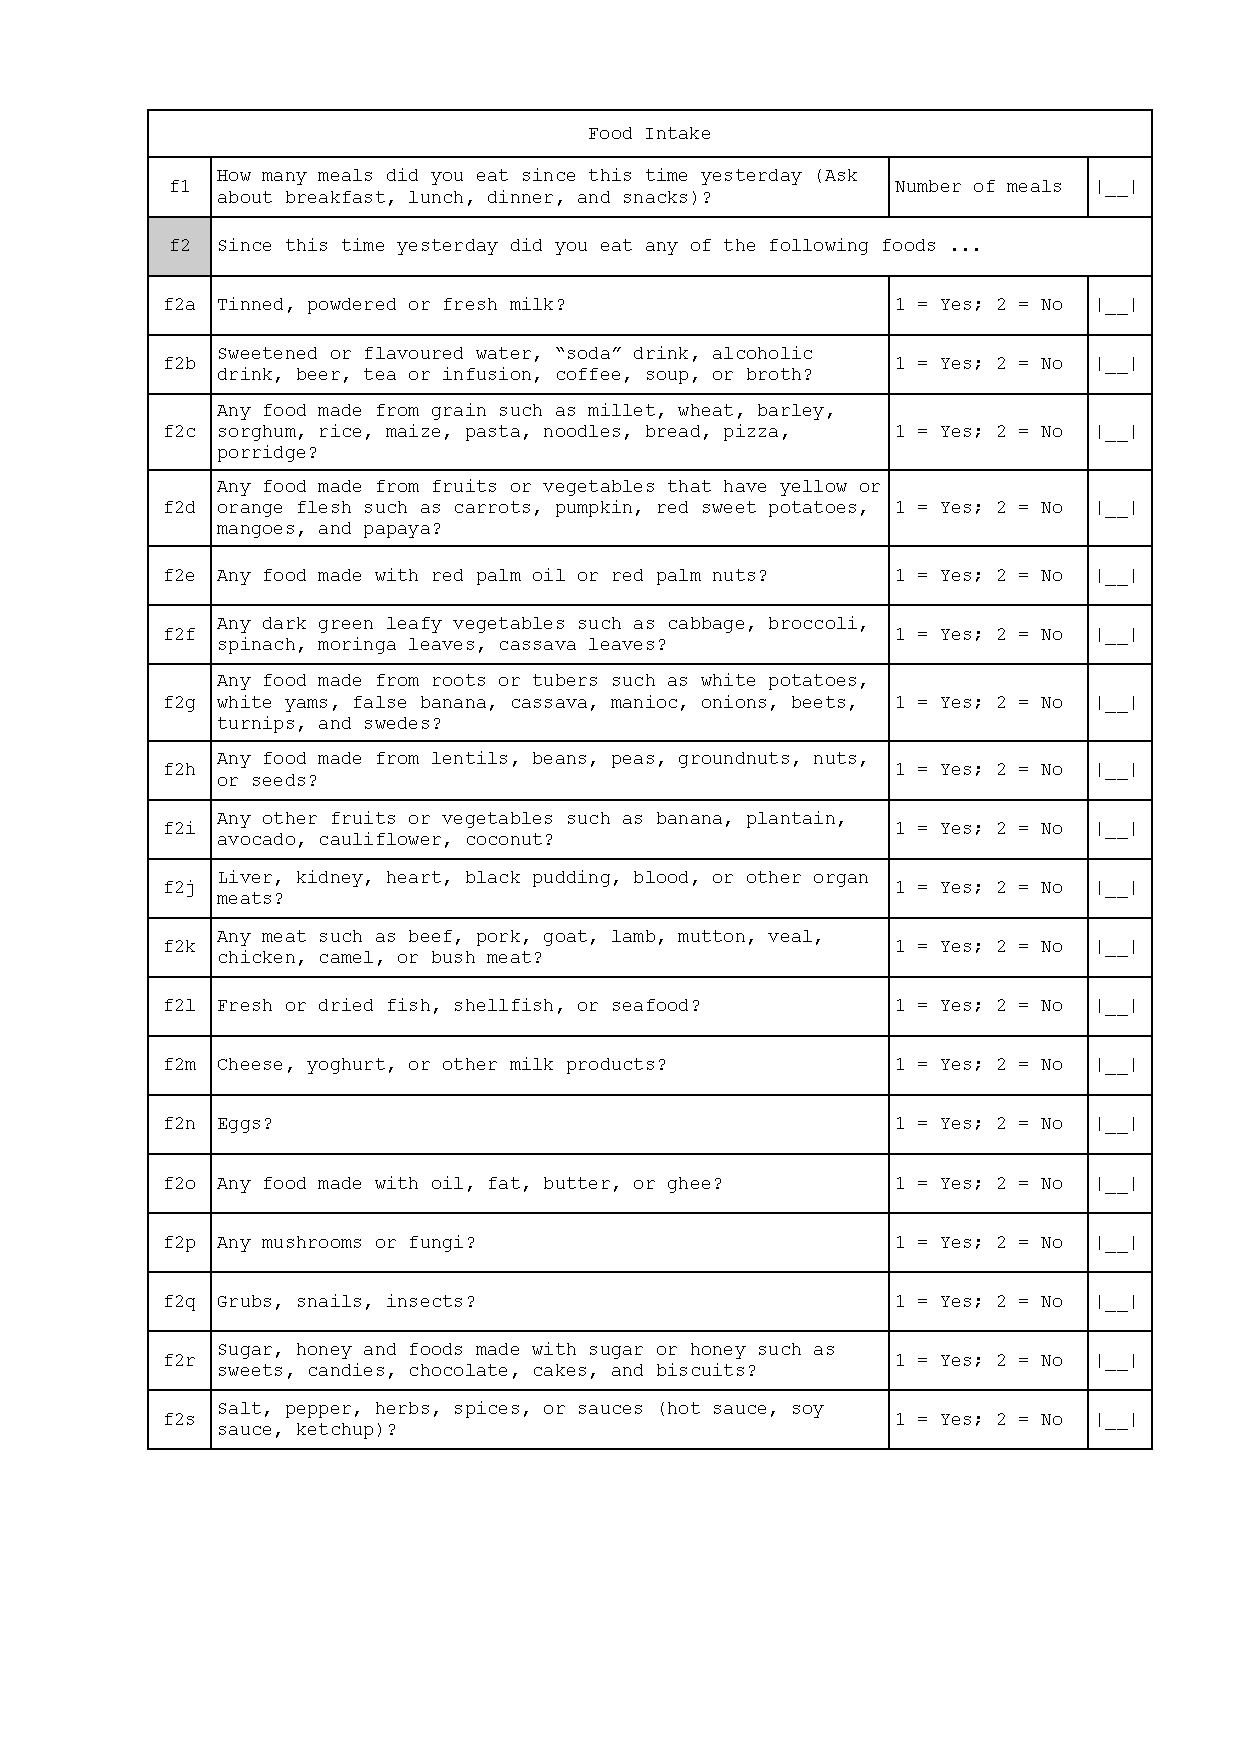
\includegraphics{figures/questionnaire02} \end{center}

\newpage

There are three related sets of diet-related indicators:

\begin{itemize}
\tightlist
\item
  meal frequency
\item
  food groups consumed / dietary diversity
\item
  indicators of nutrient consumption.
\end{itemize}

The indicator hierarchy is:

\begin{center}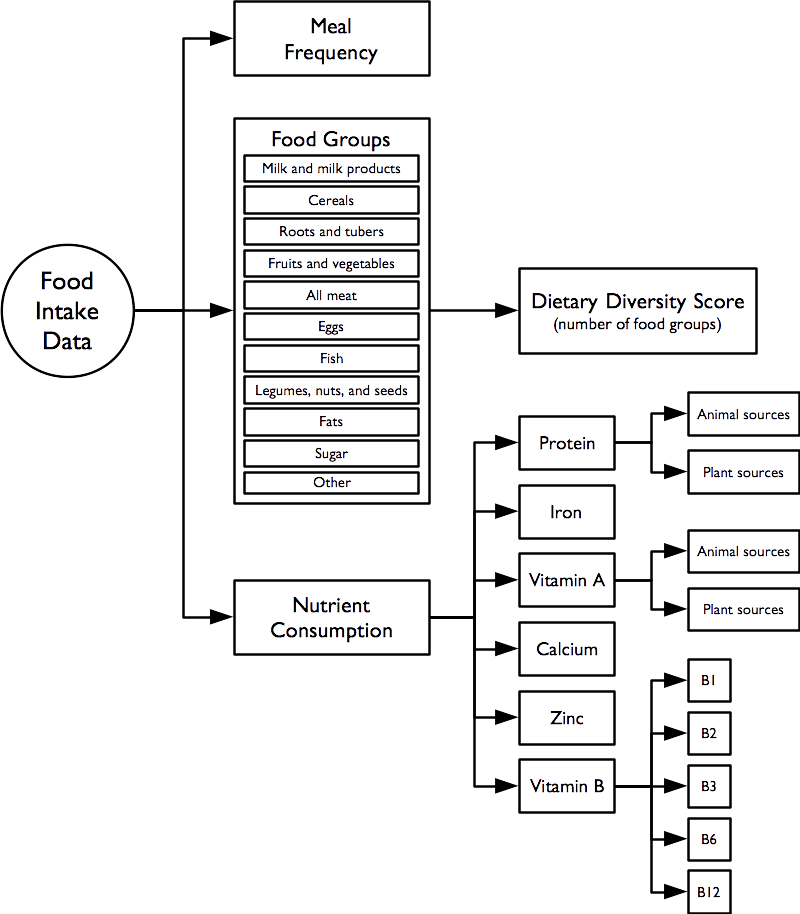
\includegraphics{figures/indicators04} \end{center}

The data on the number of meals taken in the previous twenty-four hours
forms a \emph{meal frequency score}.

Food intake data from each subject is combined into a \emph{dietary
diversity score}. The dietary diversity score is a crude measure of food
security. The dietary diversity score ranges between zero (i.e.~no food
groups) and eleven (i.e.~eleven food groups). Higher values of the
dietary diversity sore are associated with better food security.

The meal frequency score and the dietary diversity score follow:

\begin{itemize}
\item
  Swindale A, Bilinsky P, \emph{Household Dietary Diversity Score (HDDS)
  for measurement of household food access: Indicator guide}.,Washington
  DC, Food and Nutrition Technical Assistance (FANTA) Project, 2006
\item
  Kennedy G, Ballard T, Dop MC, \emph{Guidelines for Measuring Household
  and Individual Dietary Diversity}, Rome, Food and Agricultural
  Organization, 2010
\end{itemize}

The data on the types of food consumed in the previous twenty-four hours
are analysed in order to determine the diet's content of specific
micronutrients that are important for older people. This also follows
Swindale \& Bilinsky (2006) and Kennedy et al (2010), and:

\begin{itemize}
\tightlist
\item
  World Health Organisation, \emph{The management of nutrition in major
  emergencies}, Geneva, WHO, 2000
\end{itemize}

\hypertarget{meal-frequency}{%
\subsection{Meal frequency}\label{meal-frequency}}

The meal frequency score indicator is the answer given to the first food
intake question:

\begin{center}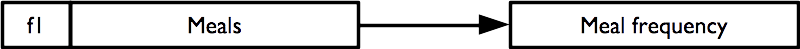
\includegraphics{figures/indicators05} \end{center}

Meal frequency is a crude measure of food security.

Higher values of meal frequency are associated with better food
security.

\hypertarget{food-groups-and-dietary-diversity}{%
\subsection{Food groups and dietary
diversity}\label{food-groups-and-dietary-diversity}}

Questions relating to the consumption of individual food items / food
types are combined to create food groups and the number of food groups
consumed are counted to create a dietary diversity score:

\begin{center}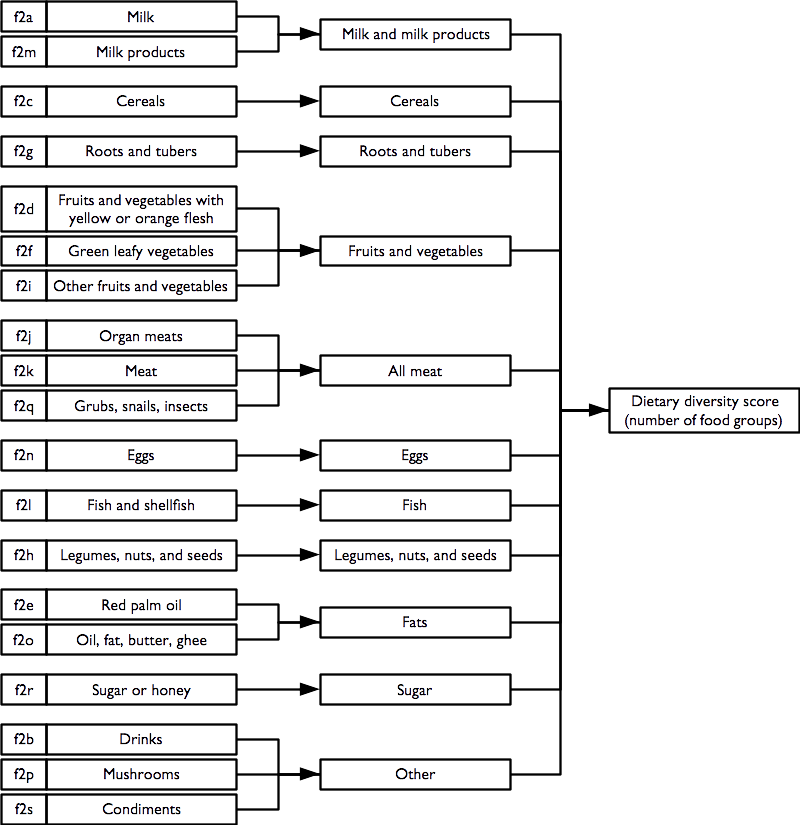
\includegraphics{figures/indicators06} \end{center}

The consumption of the eleven individual food groups and the dietary
diversity score are reported separately.

The dietary diversity score is a crude measure of food security. The
dietary diversity score ranges between zero (no food groups) and eleven
(eleven food groups). Higher values of the dietary diversity score are
associated with better food security.

\hypertarget{indicators-of-nutrient-consumption}{%
\subsection{Indicators of nutrient
consumption}\label{indicators-of-nutrient-consumption}}

\textbf{Overview}

Questions and combinations of questions relating to the consumption of
individual food items and food types can be used to determine whether
the reported diet is likely to be provide sufficient nutrients of
various types:

\begin{center}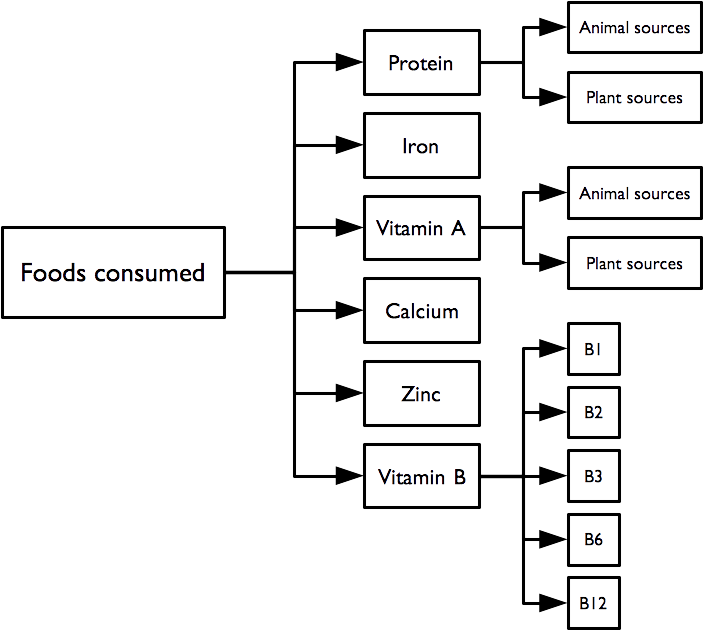
\includegraphics{figures/indicators07} \end{center}

Each indicator is formed using logical ``or'' operations (i.e.~the
indicator is true if \textbf{any} of the constituent foods are
consumed). For example, the indicator for the consumption of iron rich
foods:

\begin{center}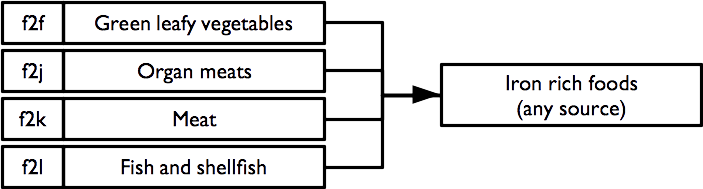
\includegraphics{figures/indicators08} \end{center}

requires the consumption of one or more of green leafy vegetables, organ
meats, meat, or fish and shellfish. Consumption of \textbf{any} of these
foods is sufficient to indicate that the survey subject consumes iron
rich food.

\hypertarget{protein-rich-foods}{%
\subsubsection{Protein rich foods}\label{protein-rich-foods}}

Indicators of consumption of protein rich foods from animal sources,
plant source, and any / all sources are calculated as:

\begin{center}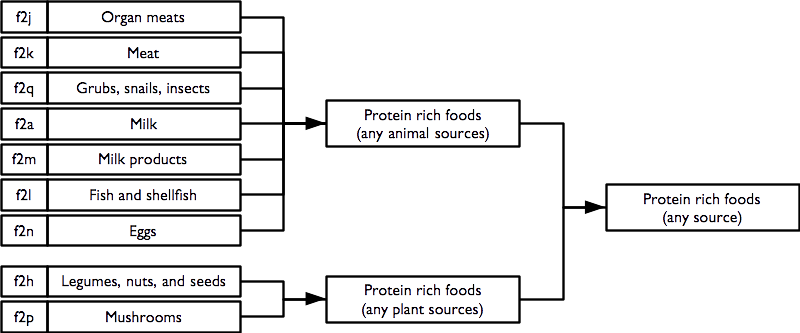
\includegraphics{figures/indicators09} \end{center}

\hypertarget{vitamin-a-rich-foods}{%
\subsubsection{Vitamin A rich foods}\label{vitamin-a-rich-foods}}

Indicators of consumption of vitamin A rich foods from animal sources,
plant source, and any / all sources are calculated as:

\begin{center}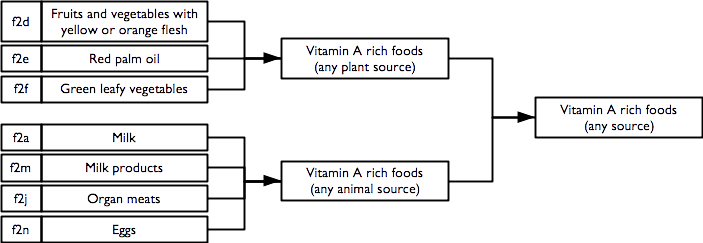
\includegraphics{figures/indicators10} \end{center}

\newpage

\hypertarget{iron-rich-foods}{%
\subsubsection{Iron rich foods}\label{iron-rich-foods}}

An indicator of consumption of iron rich foods from any / all sources is
calculated as:

\begin{center}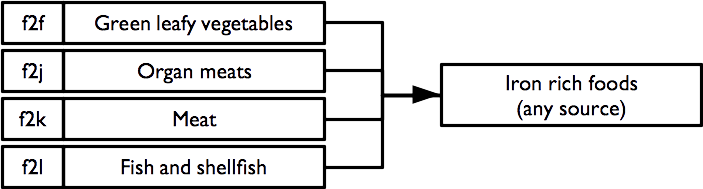
\includegraphics{figures/indicators11} \end{center}

\hypertarget{calcium-rich-foods}{%
\subsubsection{Calcium rich foods}\label{calcium-rich-foods}}

An indicator of consumption of calcium rich foods from any / all sources
is calculated as:

\begin{center}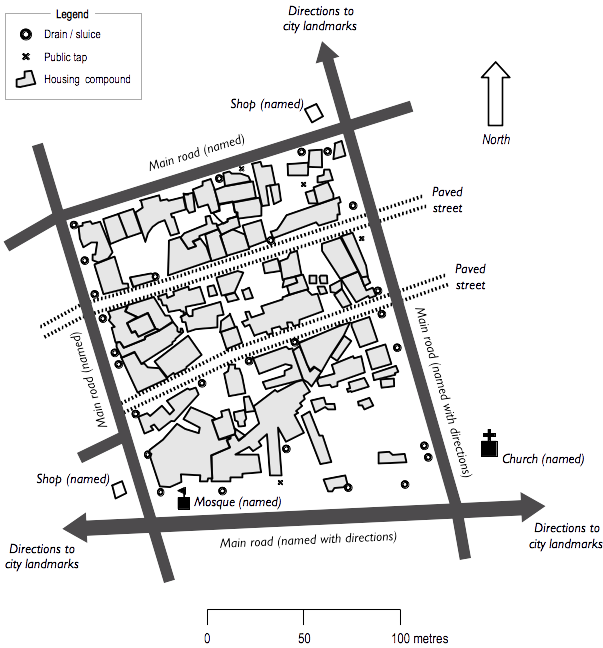
\includegraphics{figures/indicators12} \end{center}

\hypertarget{zinc-rich-foods}{%
\subsubsection{Zinc rich foods}\label{zinc-rich-foods}}

An indicator of consumption of zinc rich foods from any / all sources is
calculated as:

\begin{center}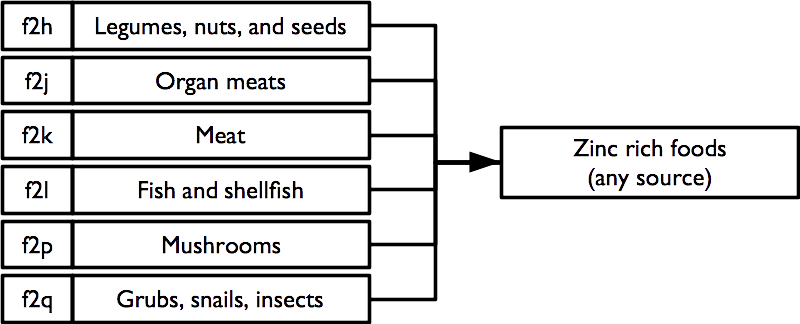
\includegraphics{figures/indicators13} \end{center}

\newpage

\hypertarget{vitamin-b-rich-foods}{%
\subsubsection{Vitamin B rich foods}\label{vitamin-b-rich-foods}}

Indicators of consumption of vitamin B rich foods from any / all sources
are calculated as:

\begin{center}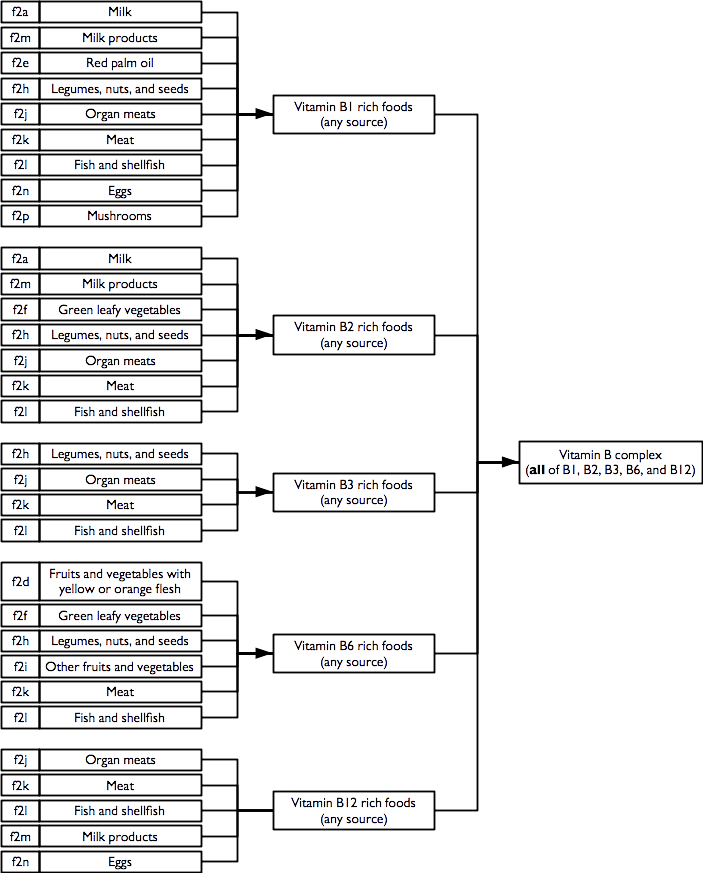
\includegraphics{figures/indicators14} \end{center}

Note that the vitamin B complex indicator requires that at least one
food from each of the B1, B2, B3, B6, and B12 rich food combinations is
consumed.

\hypertarget{severe-food-insecurity}{%
\subsection{Severe food insecurity}\label{severe-food-insecurity}}

An indicator of severe food insecurity (hunger) is derived from this
questionnaire component:

\begin{center}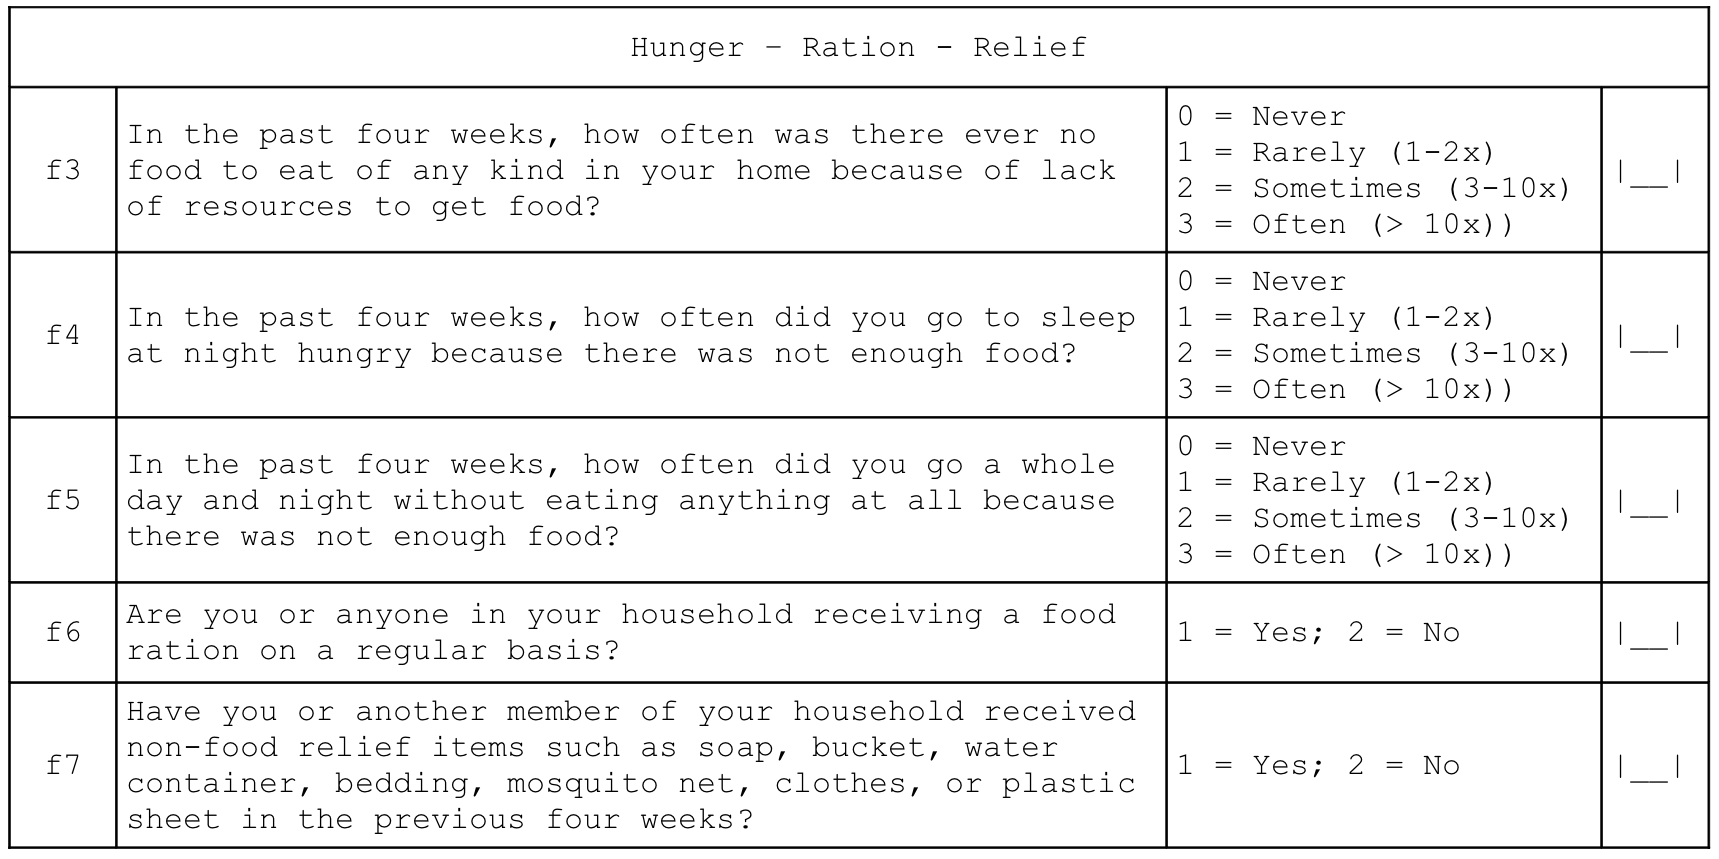
\includegraphics{figures/questionnaire03} \end{center}

and is calculated as:

\begin{center}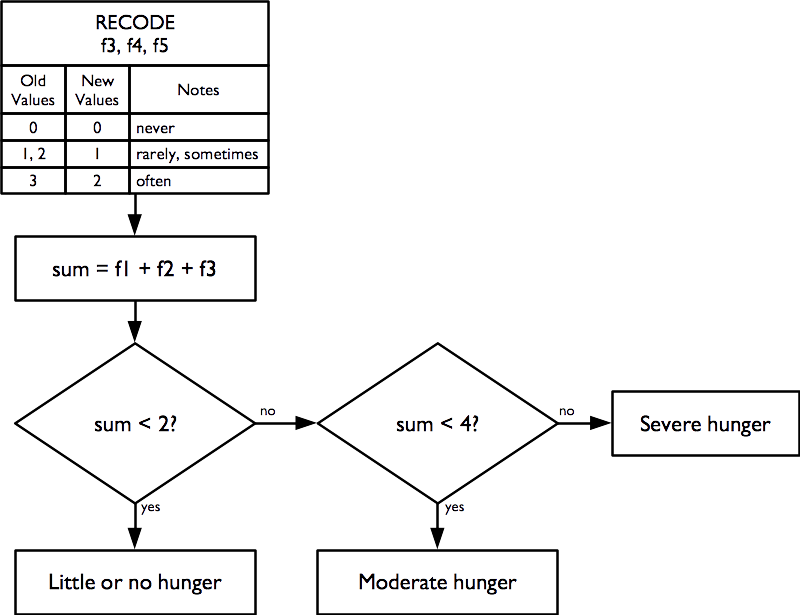
\includegraphics{figures/indicators15} \end{center}

\newpage

This indicator is the \emph{Household Hunger Scale (HHS)} and is a
simple, well-validated, and widely used indicator of severe food
insecurity:

\begin{itemize}
\item
  Ballard T, Coates J, Swindale A, Deitchler M, \emph{Household Hunger
  Scale: Indicator Definition and Measurement Guide}, Washington DC,
  FANTA-2 Bridge, FHI 360, 2011
\item
  Ruel MT, Ballard TJ, Deitchler M, \emph{Measuring and Tracking the
  Access Dimension of Food Security: Available Indicators and
  Recommendations for Future Investments}, Global Nutrition Report 2014:
  Technical Note 6, Washington DC, International Food Policy Research
  Institute, 2014
\end{itemize}

\hypertarget{disability}{%
\subsection{Disability}\label{disability}}

Indicators of disability across six different domains are derived from
this questionnaire component:

\begin{center}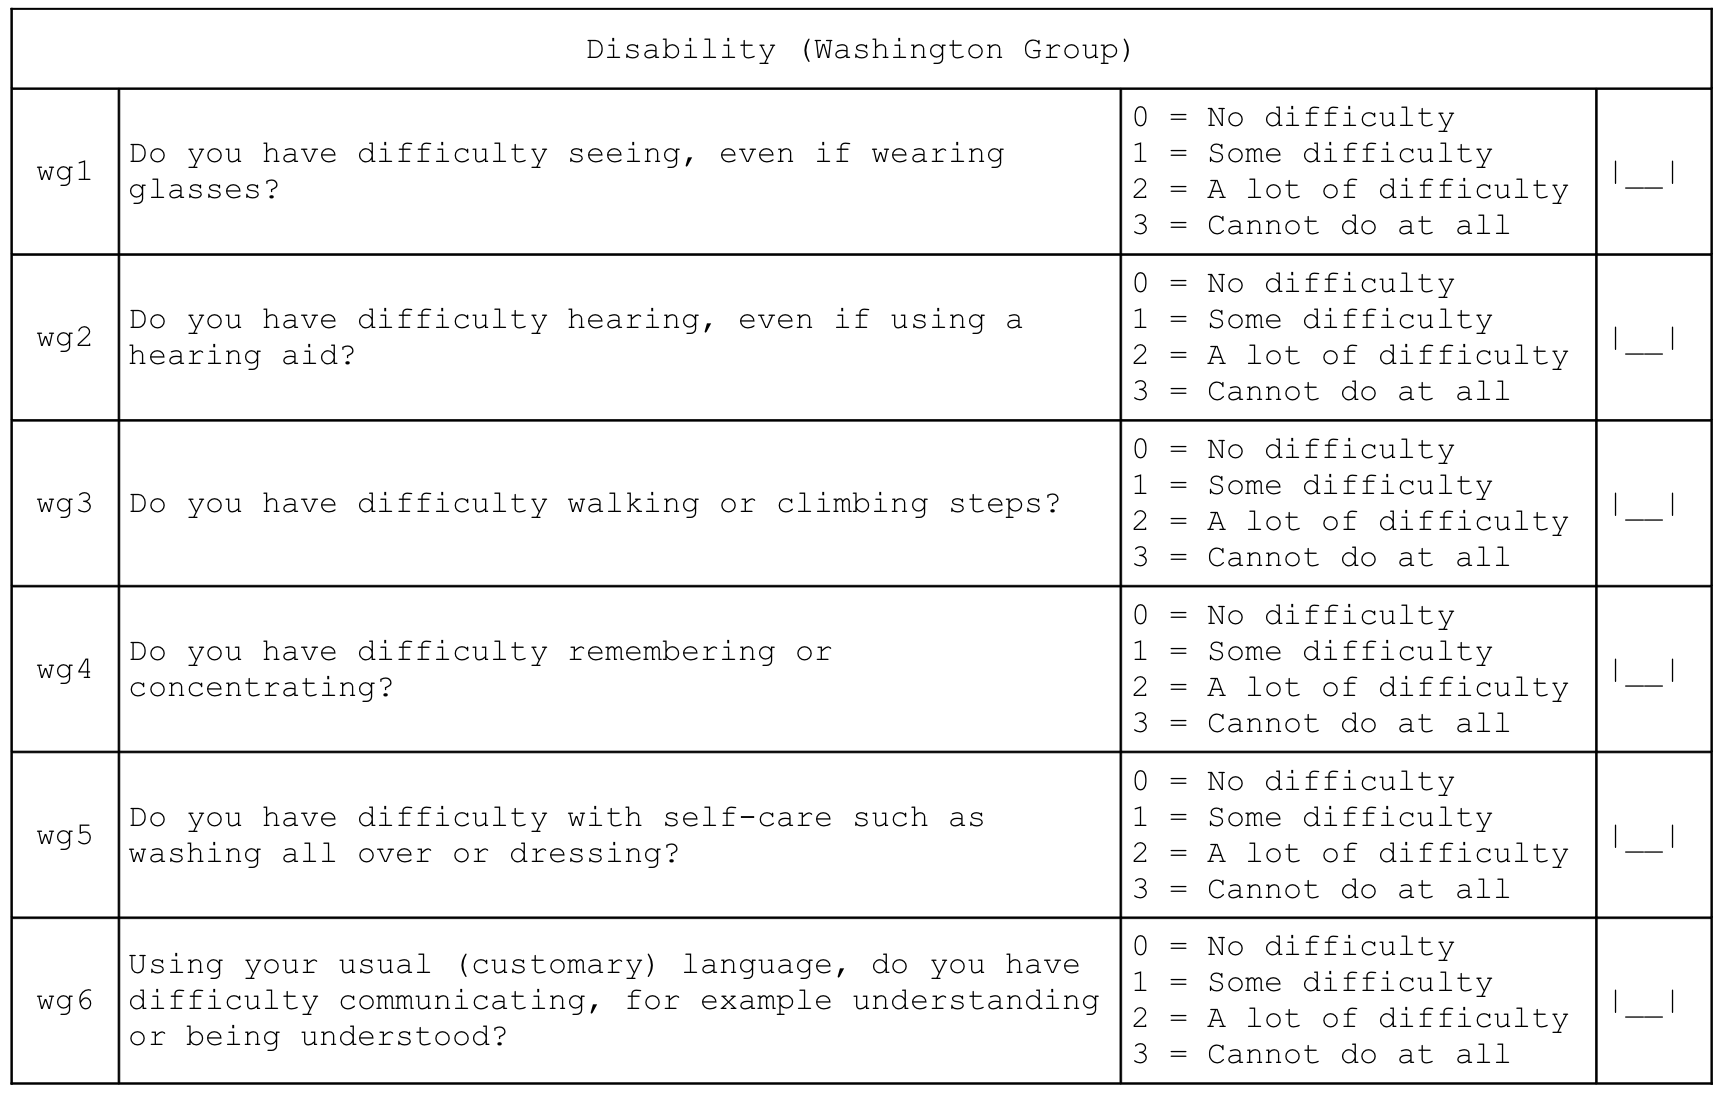
\includegraphics{figures/questionnaire04} \end{center}

\newpage

Individual disability indicators are reported for each domain
(i.e.~vision, hearing, mobility, remembering, self-care, and
communication) of disability in the Washington Group's short set of
question designed to identify people with a disability in a census or
survey format:

\begin{itemize}
\item
  \url{http://www.washingtongroup-disability.com}
\item
  \url{https://www.cdc.gov/nchs/washington_group/wg_documents.htm}
\end{itemize}

Overall disability prevalence indicators are also reported.

Indicators of disability in each domain are calculated as:

\begin{center}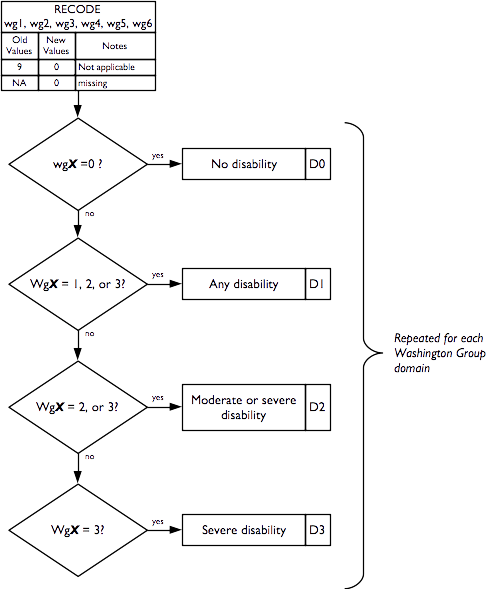
\includegraphics{figures/indicators16} \end{center}

Overall disability prevalence indicators are calculated as:

\begin{longtable}[]{@{}ll@{}}
\toprule
\begin{minipage}[t]{0.11\columnwidth}\raggedright
\texttt{P0} = 1\strut
\end{minipage} & \begin{minipage}[t]{0.83\columnwidth}\raggedright
if no domain has \texttt{D1} = 1, else = 0 (no disability in any
domain)\strut
\end{minipage}\tabularnewline
\begin{minipage}[t]{0.11\columnwidth}\raggedright
\texttt{P1} = 1\strut
\end{minipage} & \begin{minipage}[t]{0.83\columnwidth}\raggedright
if at least one domain has \texttt{D1} = 1, else = 0\strut
\end{minipage}\tabularnewline
\begin{minipage}[t]{0.11\columnwidth}\raggedright
\texttt{P2} = 1\strut
\end{minipage} & \begin{minipage}[t]{0.83\columnwidth}\raggedright
if at least one domain has \texttt{D2} = 1, else = 0\strut
\end{minipage}\tabularnewline
\begin{minipage}[t]{0.11\columnwidth}\raggedright
\texttt{P3} = 1\strut
\end{minipage} & \begin{minipage}[t]{0.83\columnwidth}\raggedright
if at least one domain has \texttt{D3} = 1, else = 0\strut
\end{minipage}\tabularnewline
\begin{minipage}[t]{0.11\columnwidth}\raggedright
\texttt{PM} = 1\strut
\end{minipage} & \begin{minipage}[t]{0.83\columnwidth}\raggedright
if at more than one domain has \texttt{D1} = 1, else = 0 (M stands for
``Multiple'')\strut
\end{minipage}\tabularnewline
\bottomrule
\end{longtable}

\hypertarget{activities-of-daily-living}{%
\subsection{Activities of daily
living}\label{activities-of-daily-living}}

Indicators of how well the subject copes with activities of daily living
are derived from this questionnaire component:

\begin{center}\includegraphics{figures/questionnaire05} \end{center}

Individual \emph{independence} indicators are reported for each
dimension (i.e.~bathing, dressing, toilet, mobility, continence, and
eating) of daily living activities.

A composite indicator of the degree of \emph{independence} (i.e.~how
well the subject can cope with activities of daily living) is also
reported. This indicator is the \emph{Katz Index of Independence in
Activities of Daily Living} (or the \emph{Katz Index of ADL} for short)
and is a simple, well-validated, and widely used indicator of how well
the subject can cope with activities of daily living:

\begin{itemize}
\item
  Katz S, Ford AB, Moskowitz RW, Jackson BA, Jaffe MW, \emph{Studies of
  illness in the aged. The Index of ADL: A standardized measure of
  biological and psychosocial function}, JAMA, 185(12), 1963, pp.~914-9
\item
  Katz S, Down TD, Cash HR, Grotz, RC, \emph{Progress in the development
  of the index of ADL}, The Gerontologist, 10(1), 1970, pp.~20-30
\item
  Katz S, \emph{Assessing self-maintenance: Activities of daily living,
  mobility and instrumental activities of daily living}, JAGS, 31(12),
  1983, pp.~721-726
\end{itemize}

The Katz Index of ADL ranges between zero (complete dependence) and six
(independence).

\newpage

The seventh question of this module, which is not part of the Katz Index
of ADL, is reported separately and indicates whether the subject has
someone to help them with activities of daily living:

\begin{longtable}[]{@{}c@{}}
\toprule
\begin{minipage}[t]{0.97\columnwidth}\centering
\textbf{Activities of Daily Living}\strut
\end{minipage}\tabularnewline
\bottomrule
\end{longtable}

\begin{longtable}[]{@{}llll@{}}
\toprule
\begin{minipage}[t]{0.09\columnwidth}\raggedright
a7\strut
\end{minipage} & \begin{minipage}[t]{0.41\columnwidth}\raggedright
Is someone taking care of you or helping you with everyday activities
such as shopping, cooking, bathing and dressing?\strut
\end{minipage} & \begin{minipage}[t]{0.25\columnwidth}\raggedright
1 = Yes; 2 = No\strut
\end{minipage} & \begin{minipage}[t]{0.13\columnwidth}\raggedright
{[}\_\_{]}\strut
\end{minipage}\tabularnewline
\bottomrule
\end{longtable}

It is not possible to know if the help available completely meets a
subject's needs, but we can identify the proportion of subjects needing
help with one or more activities of daily living who also report not
having someone to help them:

\begin{center}\includegraphics{figures/indicators17} \end{center}

This is an indicator of unmet need.

\newpage

Indicators of how well the subject can cope with activities of daily
living and probable unmet need are calculated as:

\begin{center}\includegraphics{figures/indicators18} \end{center}

\hypertarget{mental-health-and-well-being}{%
\subsection{Mental health and
well-being}\label{mental-health-and-well-being}}

Indicators of mental health and well being are derived from this
questionnaire component:

\begin{center}\includegraphics{figures/questionnaire06} \end{center}

A score is calculated. This is the \emph{Kessler K6 Psychological
Distress Scale}. The score ranges from zero (indicating no psychological
distress) to twenty-four (indicating severe psychological distress). A
score of thirteen or more indicates serious psychological distress. The
Kessler K6 Psychological Distress Scale is a widely recommended, widely
used, accurate, reliable, and simple measure of psychological distress:

\begin{itemize}
\item
  Kessler RC, Andrews G, Colpe LJ, Hiripi E, Mroczek, DK, Normand SLT,
  et al, ``Short screening scales to monitor population prevalences and
  trends in non-specific psychological distress'', \emph{Psychological
  Medicine}, 32(6), 2002, pp.~959--976
\item
  Kessler RC, Barker PR, Colpe LJ, Epstein JF, Gfroerer JC, Hiripi E,
  ``Screening for Serious Mental Illness in the General Population'',
  \emph{Archives of General Psychiatry}, 60(2), 2003, pp.~184-189
\end{itemize}

Indicators of mental health and well-being are calculated as:

\begin{center}\includegraphics{figures/indicators19} \end{center}

\newpage

\hypertarget{dementia}{%
\subsection{Dementia}\label{dementia}}

An indicator of probable dementia is derived from this questionnaire
component:

\begin{center}\includegraphics{figures/questionnaire07} \end{center}

\newpage

The indicator of \emph{probable} dementia is calculated as:

\begin{center}\includegraphics{figures/indicators20} \end{center}

This indicator is derived from the Community Screening Instrument for
Dementia (CSID) developed by the 10/66 Dementia Research Group. This is
a simple, validated, and widely used indicator of probable dementia:

\begin{itemize}
\tightlist
\item
  Prince M, et al, ``A brief dementia screener suitable for use by
  non-specialists in resource poor settings - The cross-cultural
  derivation and validation of the brief Community Screening Instrument
  for Dementia'', \emph{International Journal of Geriatric Psychiatry},
  26(9), 2011, pp.~899--907
\end{itemize}

\newpage

\hypertarget{health-and-health-seeking-behaviour}{%
\subsection{Health and health-seeking
behaviour}\label{health-and-health-seeking-behaviour}}

Indicators of health and health-seeking behaviour for chronic and acute
conditions are derived from this questionnaire component:

\begin{center}\includegraphics{figures/questionnaire08} \end{center}

\newpage

Indicators of health and health-seeking behaviour for chronic conditions
are calculated as:

\begin{center}\includegraphics{figures/indicators21} \end{center}

\newpage

Indicators of health and health-seeking behaviour for acute conditions
are calculated as:

\begin{center}\includegraphics{figures/indicators22} \end{center}

\hypertarget{sources-of-income}{%
\subsection{Sources of income}\label{sources-of-income}}

Indicators related to sources of income are derived from this
questionnaire component:

\begin{center}\includegraphics{figures/questionnaire09} \end{center}

and are calculated as:

\begin{center}\includegraphics{figures/indicators23} \end{center}

\newpage

The grouped income sources (i.e. \texttt{m2a}, \texttt{m2b}, etc.) and
individual income sources may vary between settings. The questionnaire
component shown above has proved suitable for use in Ethiopia, South
Sudan, and Tanzania.

\hypertarget{water-sanitation-and-hygiene}{%
\subsection{Water, sanitation, and
hygiene}\label{water-sanitation-and-hygiene}}

Indicators relating to water, sanitation, and hygiene (WASH) are derived
from this questionnaire component:

\begin{center}\includegraphics{figures/questionnaire10} \end{center}

\newpage

Indicators are calculated following:

\begin{itemize}
\tightlist
\item
  WHO / UNICEF, \emph{Core Questions on Drinking-water and Sanitation
  for Household Surveys}, Geneva, WHO / UNICEF, 2006
\end{itemize}

\newpage

Indicators relating to water, sanitation, and hygiene (WASH) are
calculated as:

\begin{center}\includegraphics{figures/indicators24} \end{center}

\hypertarget{anthropometry-and-screening-coverage}{%
\subsection{Anthropometry and screening
coverage**}\label{anthropometry-and-screening-coverage}}

Indicators relating to anthropometry and screening coverage are derived
from this questionnaire component:

\begin{center}\includegraphics{figures/questionnaire11} \end{center}

\newpage

And are calculated as:

\begin{center}\includegraphics{figures/indicators25} \end{center}

Raw MUAC data (i.e.~not MUAC class) is collected, entered, and analysed.
This requires that an adult MUAC tape (i.e.~capable of measuring MUAC to
450 mm) is used.

The presence of bilateral oedema is assessed by pressing with your
thumbs \textbf{both} feet of the older person for three seconds and
checking whether this creates a lasting depression or ``pit'' on both
feet. Bilateral pitting oedema in older people may not be
``nutritional'' oedema (as is almost always the case with children).
Older people with bilateral pitting oedema should be advised to consult
a doctor.

The prevalence of GAM, MAM, and SAM are estimated using a PROBIT
estimator. This type of estimator provides better precision than a
classic estimator at small sample sizes:

\begin{itemize}
\item
  World Health Organisation, \emph{Physical Status: The use and
  interpretation of anthropometry. Report of a WHO expert committee},
  WHO Technical Report Series 854, WHO, Geneva, 1995
\item
  Dale NM, Myatt M, Prudhon C, Briend, A, ``Assessment of the PROBIT
  approach for estimating the prevalence of global, moderate and severe
  acute malnutrition from population surveys'', \emph{Public Health
  Nutrition}, 1--6. \url{doi:10.1017/S1368980012003345}, 2012
\item
  Blanton CJ, Bilukha, OO, ``The PROBIT approach in estimating the
  prevalence of wasting: revisiting bias and precision'', \emph{Emerging
  Themes in Epidemiology}, 10(1), 2013, p.~8
\end{itemize}

The PROBIT estimator is described in Box 1.

MUAC-based case definitions for acute malnutrition are used:

\begin{longtable}[]{@{}ll@{}}
\toprule
\begin{minipage}[t]{0.14\columnwidth}\raggedright
\textbf{GAM}\strut
\end{minipage} & \begin{minipage}[t]{0.31\columnwidth}\raggedright
:\textbar{} MUAC \textless{} 210 mm\strut
\end{minipage}\tabularnewline
\begin{minipage}[t]{0.14\columnwidth}\raggedright
\textbf{MAM}\strut
\end{minipage} & \begin{minipage}[t]{0.31\columnwidth}\raggedright
:\textbar{} 185 mm ≤ MUAC \textless{} 210mm\strut
\end{minipage}\tabularnewline
\begin{minipage}[t]{0.14\columnwidth}\raggedright
\textbf{SAM}\strut
\end{minipage} & \begin{minipage}[t]{0.31\columnwidth}\raggedright
:\textbar{} MUAC \textless{} 185mm\strut
\end{minipage}\tabularnewline
\bottomrule
\end{longtable}

These are standard case definitions for acute malnutrition in adults and
recommended by HelpAge International for use in older people in
humanitarian contexts.

\textbf{Note} : MUAC in adults should be measured on the non-dominant
arm. This is usually the left arm. The importance of high levels of
accuracy and precision at the individual level is of lesser importance
in survey work compared to case-finding or diagnosis in clinical
contexts, for example. This means that a simple rule such as ``Always
measure MUAC on the left arm'' may be used.

\newpage

\BeginKnitrBlock{rmdexercise}
An estimate of GAM prevalence can be made using a classic estimator:

\[\text{prevalence} = \frac{\text{number of respondents with MUAC < 210 mm}}{\text{total number of respondents}}\]

The estimate of GAM prevalence made from the RAM-OP survey data is made
using a PROBIT estimator. The PROBIT function is also known as the
\emph{inverse cumulative distribution} function. This function converts
parameters of the distribution of an indicator (e.g.~the mean and
standard deviation of a \emph{normally} distributed variable) into
cumulative percentiles. This means that it is possible to use the normal
PROBIT function with estimates of the mean and standard deviation of
indicator values in a survey sample to predict (or estimate) the
proportion of the population falling below a given threshold. For
example, for data with a mean MUAC of 256 mm and a standard deviation of
28 mm the output of the normal PROBIT function for a threshold of 210 mm
is 0.0502 meaning that 5.02\% of the population are \emph{predicted} (or
\emph{estimated}) to fall below the 210 mm threshold.

Both the classic and the PROBIT methods can be thought of as estimating
area:

\includegraphics{figures/indicators26.png}

The principal advantage of the PROBIT approach is that the required
sample size is usually smaller than that required to estimate prevalence
with a given precision using the classic method.

The PROBIT method assumes that MUAC is a normally distributed variable.
If this is not the case then the distribution of MUAC is transformed
towards normality.

The prevalence of SAM is estimated in a similar way to GAM. The
prevalence of MAM is estimated as the difference between the GAM and SAM
prevalence estimates:

\[\widehat{MAM prevalence} = \widehat{GAM prevalence} - \widehat{SAM prevalence}\]
\EndKnitrBlock{rmdexercise}

\newpage

\hypertarget{visual-impairment}{%
\subsection{Visual impairment}\label{visual-impairment}}

An indicator of visual impairment is derived from this questionnaire
component:

\begin{center}\includegraphics{figures/questionnaire12} \end{center}

And is calculated as:

\begin{center}\includegraphics{figures/indicators27} \end{center}

The ``illiterate E'' or ``tumbling E'' (the preferred term) is a
validated and widely used method for measuring visual acuity:

\begin{itemize}
\item
  Taylor HR, ``Applying new design principles to the construction of an
  illiterate E chart'', \emph{American Journal of Optometry \&
  Physiological Optics}, 55:348, 1978
\item
  Kaiser PK, ``Prospective Evaluation of Visual Acuity Assessment: A
  Comparison of Snellen Versus ETDRS Charts in Clinical Practice (An AOS
  Thesis)'', \emph{Transactions of the American Ophthalmological
  Society}, 107: 311--324, 2009
\end{itemize}

The size of the ``E'' used:

\begin{center}\includegraphics{figures/indicators28} \end{center}

as well as the distance used for the test (two metres) and the indicator
calculation apply the WHO case definition of visual impairment
(i.e.~visual acuity \textless{} 6 / 18).

The tumbling E card should be laminated (i.e.~plastic coated and have a
two metre cord attached which helps to ensure that the visual acuity
test is performed at the correct distance (See Figure
\ref{fig:indicators29}).

After demonstrating to the respondent what the test is about (i.e.~the
subject should indicate which direction the branches of the `E' are
pointing), the test is administered at a distance of two meters, turning
the card in four different directions, and asking the person to indicate
which direction the branches of the ``E'' is pointing. If the subject
wears glasses, they are allowed to use them during the test if they want
to.

\textbf{Note} : If the person is unable to correctly answer at least
three times out of four, they have a visual impairment. A simple visual
acuity test such as the `tumbling E' test also does not indicate
anything about an underlying disease such as glaucoma or the need for
reading spectacles (presbyopia). These conditions are common in people
aged 60 years or older. Subjects failing the visual acuity test should
be counselled to visit an ophthalmologist for a detailed eye
examination.

\begin{figure}[H]

{\centering \includegraphics{figures/indicators29} 

}

\caption{Equipment used to measure visual acuity}\label{fig:indicators29}
\end{figure}

\hypertarget{miscellaneous-indicators}{%
\subsection{Miscellaneous indicators}\label{miscellaneous-indicators}}

Data for a small group of miscellaneous indicators are also collected
and reported. These are derived from these questions:

\begin{longtable}[]{@{}c@{}}
\toprule
\begin{minipage}[t]{0.97\columnwidth}\centering
\textbf{Hunger -- Ration - Relief}\strut
\end{minipage}\tabularnewline
\bottomrule
\end{longtable}

\begin{longtable}[]{@{}llll@{}}
\toprule
\begin{minipage}[t]{0.09\columnwidth}\raggedright
f6\strut
\end{minipage} & \begin{minipage}[t]{0.41\columnwidth}\raggedright
Are you or anyone in your household receiving a food ration on a regular
basis?\strut
\end{minipage} & \begin{minipage}[t]{0.25\columnwidth}\raggedright
1 = Yes; 2 = No\strut
\end{minipage} & \begin{minipage}[t]{0.13\columnwidth}\raggedright
{[}\_\_{]}\strut
\end{minipage}\tabularnewline
\begin{minipage}[t]{0.09\columnwidth}\raggedright
f7\strut
\end{minipage} & \begin{minipage}[t]{0.41\columnwidth}\raggedright
Have you or another member of your household received non-food relief
items such as soap, bucket, water container, bedding, mosquito net,
clothes, or plastic sheet in the previous four weeks?\strut
\end{minipage} & \begin{minipage}[t]{0.25\columnwidth}\raggedright
1 = Yes; 2 = No\strut
\end{minipage} & \begin{minipage}[t]{0.13\columnwidth}\raggedright
{[}\_\_{]}\strut
\end{minipage}\tabularnewline
\bottomrule
\end{longtable}

\begin{longtable}[]{@{}c@{}}
\toprule
\begin{minipage}[t]{0.97\columnwidth}\centering
\textbf{Activities of Daily Living}\strut
\end{minipage}\tabularnewline
\bottomrule
\end{longtable}

\begin{longtable}[]{@{}llll@{}}
\toprule
\begin{minipage}[t]{0.09\columnwidth}\raggedright
a8\strut
\end{minipage} & \begin{minipage}[t]{0.41\columnwidth}\raggedright
Do you have problems chewing food?\strut
\end{minipage} & \begin{minipage}[t]{0.25\columnwidth}\raggedright
1 = Yes; 2 = No\strut
\end{minipage} & \begin{minipage}[t]{0.13\columnwidth}\raggedright
{[}\_\_{]}\strut
\end{minipage}\tabularnewline
\bottomrule
\end{longtable}

and are calculated as:

\begin{center}\includegraphics{figures/indicators30} \end{center}

\hypertarget{a-note-on-data-management-and-data-analysis}{%
\section{A note on data management and data
analysis}\label{a-note-on-data-management-and-data-analysis}}

This section has described how RAM-OP data is used to create a broad set
of indicators. If you do not want to use the standard RAM-OP software to
do this then you can use this information to create data entry systems
and data management scripts for your favoured database or statistical
analysis software. See the sections on
\protect\hyperlink{datasets}{\textbf{RAM-OP datasets}} and
\protect\hyperlink{questionnaire}{\textbf{RAM-OP questionnaire}} for
more compact information on variable names and codes that you may find
helpful.

It is important to note that data analysis procedures need to account
for the sample design. All major statistical analysis software can do
this (details vary). There are two things to note:

\begin{itemize}
\tightlist
\item
  The RAM-OP sample is a two-stage sample. Subjects are sampled from a
  small number of primary sampling units (PSUs).
\item
  The RAM-OP sample is \textbf{not} prior weighted. This means that you
  will need to provide per-PSU sampling weights. These are usually the
  populations of the PSU.
\end{itemize}

You will need to specify this sample design to your statistical analysis
software. If you fail to do this then your analysis may produce
estimates that place undue weight to observations from smaller
communities with confidence intervals with lower than nominal coverage
(i.e.~they will be too narrow).

The standard RAM-OP software uses \emph{blocked weighted bootstrap}
estimation approach:

\begin{itemize}
\tightlist
\item
  \textbf{Blocked} : The block corresponds to the PSU or cluster.
\item
  \textbf{Weighted} : The RAM-OP sampling procedure does not use
  population proportional sampling to weight the sample prior to data
  collection as is done with SMART type surveys. This means that a
  posterior weighting procedure is required. The standard RAM-OP
  software uses a ``roulette wheel'' algorithm to weight (i.e.~by
  population) the selection probability of PSUs in bootstrap replicates.
\end{itemize}

A total of \texttt{m\textquotesingle{}} PSUs are sampled
\emph{with-replacement} from the survey dataset where
\texttt{m\textquotesingle{}} is the number of PSUs in the survey sample.
Individual records within each PSU are then sampled
\emph{with-replacement}. A total of n' records are sampled
\emph{with-replacement} from each of the selected PSUs where
\texttt{n\textquotesingle{}} is the number of individual records in a
selected PSU. The resulting collection of records replicates the
original survey in terms of both sample design and sample size. A large
number of replicate surveys are taken (the standard RAM-OP software uses
\(r = 399\) replicate surveys but this can be changed). The required
statistic (e.g.~the mean of an indicator value) is applied to each
replicate survey. The reported estimate consists of the 50th (point
estimate), 2.5th (lower 95\% confidence limit), and the 97.5th (upper
95\% confidence limit) percentiles of the distribution of the statistic
observed across all replicate surveys. The blocked weighted bootstrap
procedure is outlined in Figure \ref{fig:indicators31}.

The principal advantages of using a bootstrap estimator are:

\begin{itemize}
\tightlist
\item
  Bootstrap estimators work well with small sample sizes.
\item
  The method is \emph{non-parametric} and uses empirical rather than
  theoretical distributions. There are no assumptions of things like
  normality to worry about.
\item
  The method allows estimation of the sampling distribution of almost
  any statistic using only simple computational methods.
\end{itemize}

The standard RAM-OP data analysis software is described in the section
\protect\hyperlink{software}{\textbf{Standard RAM-OP software}}.

\begin{figure}[H]

{\centering \includegraphics{figures/bbw} 

}

\caption{The blocked weighted bootstrap used by the standard RAM-OP software}\label{fig:indicators31}
\end{figure}

\hypertarget{questionnaire}{%
\chapter{The RAM-OP questionnaire}\label{questionnaire}}

Modules of the RAM-OP questionnaire are presented in the
\protect\hyperlink{indicators}{\textbf{RAM-OP indicators}} section of
this manual. The entire RAM-OP questionnaire is presented in the
following pages. This questionnaire is composed of many tested and
validated components. The order of the questions and the format of the
questionnaire have been tested in several settings (Chad, Dadaab Camps,
South Sudan, Ethiopia, and Tanzania) over a period of three years. It is
strongly recommended that you do \textbf{not} change the questionnaire,
other than translating it into a language other than English and
necessary localisation (i.e.~adapting the questions to meet the
language, cultural, and other requirements of a specific target
population in order to ensure that the words, names, terms, and concepts
used are culturally appropriate and understandable to them), unless you
are very sure of what you are doing. Modifying the questionnaire may
have one or more of the following consequences:

\begin{itemize}
\item
  \textbf{Modifying the order of the questions or adding questions} :
  The links with the data entry, data checking, and data analysis
  software will be broken. You will have to modify the software to
  accommodate your changes.
\item
  \textbf{Modifying the variable names} : The links with the data entry,
  data checking, and data analysis software will be broken. You will
  have to modify the software to accommodate your changes.
\item
  \textbf{Modifying the content or the phrasing of questions} : All
  questions have been tested and are formulated for accuracy and
  reliability (precision). Modifying them may lead to loss of accuracy
  (bias) and precision
\end{itemize}

When translating the questionnaire you should check if validated
question sets for each indicator module are already available in your
local language. This is likely to be the case for the food intake,
severe food insecurity, activities of daily living, mental health and
well-being, dementia, water / sanitation / hygiene, and visual
impairment indicator modules. There may also be local language training
modules and guidelines available for these modules.

Localisation is recommended for:

\begin{itemize}
\tightlist
\item
  \textbf{Food groups} : Remove inappropriate foodstuffs and give
  examples of local foodstuffs.
\item
  \textbf{Income sources} : Review income types and income categories.
\end{itemize}

The question numbers used on the questionnaire are the names of
variables used in the RAM-OP data entry, data checking, and data
analysis software. Leaving these as they are will be helpful if you
intend to use the RAM-OP data-entry and data-analysis software.

The questionnaire can be downloaded (in ODT and PDF format) from
\url{http://www.brixtonhealth.com/qesRAMOP.zip}

\hypertarget{datasets}{%
\chapter{Datasets}\label{datasets}}

This section details the RAM-OP datasets. The information presented here
is of most use if you decide not to use the RAM-OP data entry and data
checking software. You might, for example, decide to enter survey data
using spreadsheet software such as Microsoft Excel. If you do this and
want to use the RAM-OP data analysis software then you will need to
export the data as a comma-separated-value (CSV) file with the same
variable names, variable types and lengths, and using the same codes as
shown in the tables in this section. For the main RAM-OP survey dataset
these are the same variable names, variable types, variable lengths,
codes, and in the same order as shown on the standard RAM-OP
questionnaire.

There are \textbf{two} RAM-OP datasets:

\begin{enumerate}
\def\labelenumi{\arabic{enumi}.}
\item
  \textbf{The main RAM-OP survey dataset} : This is the data collected
  by the survey questionnaire. The dataset definition for the main
  RAM-OP dataset is shown in Figure \ref{fig:dataset01}.
\item
  \textbf{The PSU dataset} : This a short and narrow file with one
  record per PSU and just two variables:
\end{enumerate}

\begin{longtable}[]{@{}ll@{}}
\toprule
\begin{minipage}[t]{0.11\columnwidth}\raggedright
\textbf{psu}\strut
\end{minipage} & \begin{minipage}[t]{0.83\columnwidth}\raggedright
The PSU identifier. This \textbf{must} use the same coding system used
to identify PSUs that is used in the main RAM-OP dataset.\strut
\end{minipage}\tabularnewline
\begin{minipage}[t]{0.11\columnwidth}\raggedright
\textbf{pop}\strut
\end{minipage} & \begin{minipage}[t]{0.83\columnwidth}\raggedright
The population of the PSU.\strut
\end{minipage}\tabularnewline
\bottomrule
\end{longtable}

The PSU dataset is used during data-analysis to weight data by PSU
population.

If you do not know population sizes (as might be the case in
emergencies) then you can collect this data:

\begin{itemize}
\item
  When you visit the PSU (i.e.~from community leaders or health
  centres).
\item
  When you visit the PSU as a doorway count or roof count.
\item
  Using recent satellite imagery as a roof count.
\end{itemize}

Relative population sizes can be used. If no better data is available
then it is reasonable to use a simple semi-quantitative assessment such
as:

\begin{longtable}[]{@{}lclc@{}}
\toprule
\begin{minipage}[b]{0.16\columnwidth}\raggedright
\textbf{Type of place}\strut
\end{minipage} & \begin{minipage}[b]{0.19\columnwidth}\centering
\textbf{Population range}*\strut
\end{minipage} & \begin{minipage}[b]{0.32\columnwidth}\raggedright
Features\strut
\end{minipage} & \begin{minipage}[b]{0.21\columnwidth}\centering
Record population as \ldots{}\strut
\end{minipage}\tabularnewline
\midrule
\endhead
\begin{minipage}[t]{0.16\columnwidth}\raggedright
Hamlet\strut
\end{minipage} & \begin{minipage}[t]{0.19\columnwidth}\centering
\textless{} 1,000\strut
\end{minipage} & \begin{minipage}[t]{0.32\columnwidth}\raggedright
Very small local market or no market\strut
\end{minipage} & \begin{minipage}[t]{0.21\columnwidth}\centering
1\strut
\end{minipage}\tabularnewline
\begin{minipage}[t]{0.16\columnwidth}\raggedright
Village\strut
\end{minipage} & \begin{minipage}[t]{0.19\columnwidth}\centering
1,000 -- 4,000\strut
\end{minipage} & \begin{minipage}[t]{0.32\columnwidth}\raggedright
Market and small shops serving the village and the surrounding
hamlets\strut
\end{minipage} & \begin{minipage}[t]{0.21\columnwidth}\centering
2\strut
\end{minipage}\tabularnewline
\begin{minipage}[t]{0.24\columnwidth}\raggedright
Town\strut
\end{minipage} & \begin{minipage}[t]{0.24\columnwidth}\centering
\begin{quote}
4,000
\end{quote}\strut
\end{minipage} & \begin{minipage}[t]{0.24\columnwidth}\raggedright
Large market, many shops (some specialised), guest houses, bus station,
government offices\strut
\end{minipage} & \begin{minipage}[t]{0.24\columnwidth}\centering
4\strut
\end{minipage}\tabularnewline
\bottomrule
\end{longtable}

*These ranges may need to be adjusted to match local circumstances.

The PSU dataset must be in comma-separated-value (CSV) format (see
Figure \ref{fig:dataset02}) for use with the RAM-OP data analysis
software.

\begin{figure}[H]

{\centering \includegraphics{figures/dataset01} 

}

\caption{Main RAM-OP dataset definition}\label{fig:dataset01}
\end{figure}

The RAM-OP data analysis requires that the main RAM-OP survey dataset is
supplied in either an \textbf{EpiInfo v6.xx} or \textbf{EpiData (REC)}
format or in a comma-separated-value (CSV) format file The RAM-OP data
analysis requires that the PSU dataset is supplied in a
comma-separated-value (.CSV) format file. Figure \ref{fig:dataset02}
shows an example of a PSU dataset in comma-separate-value (CSV) format.

\begin{figure}[H]

{\centering \includegraphics{figures/dataset02} 

}

\caption{An example comma-separated-value (CSV) format file (the example is for a RAM-OP PSU dataset)}\label{fig:dataset02}
\end{figure}

Note that the first line of a CSV format file gives the names of the
variables (e.g.~these are \texttt{psu} and \texttt{pop} for the PSU
dataset) separated by commas. Subsequent lines contain data with items
separated by commas and with one record per line. CSV format files can
be created using a plain text editor (e.g. \textbf{Notepad}) or with a
spreadsheet application such as \textbf{Microsoft Excel™}. If you use a
spreadsheet application then you will have to be careful:

\begin{itemize}
\item
  Variable names and data items must be separated by commas (not tab
  characters or semi-colon characters).
\item
  Numbers with decimal places must use the full-stop character as the
  decimal separator. In some settings a spreadsheet application may want
  to use the comma character as the decimal separator.
\item
  Avoid using accented characters in the names of and in the data
  entered into text variables. These characters can sometimes confuse
  the RAM-OP data analysis software. A CSV file should contain only
  plain text, number, and commas without formatting. Do \textbf{not} use
  a word processor application such as \textbf{Microsoft Word™} to
  create or edit a CSV file.
\end{itemize}

If you have problems using a CSV file then you should check and edit the
file using a plain text-editor such as \textbf{Notepad} or a dedicated
CSV editor such as Ron's Editor
(\url{http://www.ronsplace.eu/Products/RonsEditor})

Remember to backup your data before editing it.

\hypertarget{practical}{%
\chapter{Practical Fieldwork}\label{practical}}

This section is intended to guide you through the different steps
leading up to the fieldwork once the survey location has been
identified, and gives some tips on how the fieldwork might be organised.

\hypertarget{authorisations-and-clearances}{%
\section{Authorisations and
clearances}\label{authorisations-and-clearances}}

Before implementing the survey, you will need to get all the
authorisations relevant to the country in which you plan to work. These
could include:

\begin{itemize}
\item
  \textbf{Clearance from the national nutrition cluster} or the
  equivalent structure co-ordinating national assessment activities. In
  humanitarian contexts, this might be the only clearance that you will
  need at the national level.
\item
  \textbf{Ethical approval} : This is obtained from the country's
  national ethical committee (or equivalent). Some NGOs and UNOs also
  have ethical committees and you may also need to submit your survey
  plans to them for ethical approval. It may be necessary to work with
  both national and local ethical committees. The process of gaining
  ethical approval can take several months. It is important to note that
  RAM-OP surveys are needs assessments rather than experiments upon
  human subjects. This means that ethical clearance may not be required
  for RAM-OP surveys, or that it can be given by the chair of the
  appropriate ethical review committee without the need for a full
  meeting of the ethical review committee. It is a good idea to check
  this with the chair of the appropriate committees to see if
  permissions can be expedited. Getting ethical clearance is often very
  useful when applying for other permission as it shows that some
  technical quality assurance has been done.
\item
  \textbf{Authorisation from the appropriate government departments} at
  various levels (i.e.~national, regional, and at the level where you
  are going to implement the survey). Authorisation of the authority
  managing the survey site should be sought. For example, a survey in a
  refugee camp will need the authorisation of UNHCR, the national
  administrative authority in charge of refugees and displaced persons,
  and the agency in charge of the camp management. In some settings you
  may also need to obtain authorisation from other government
  departments such as the Ministry of Health, the Department of Rural
  Affairs, or the Department of Social Affairs.
\item
  \textbf{Authorisation from the administrative authorities at local
  level} : Make sure that all levels of the local administration are
  informed about what you intend to do (i.e.~what, where, and when). It
  is essential to meet with the local administrative and health
  authorities prior to the survey. This is done to avoid problems with
  permissions and to involve them in the implementation of the survey.
  Describe the survey and explain what might be expected from their
  staff. You might, for example, need some help in identifying the exact
  location and boundaries of villages and hamlets in rural areas, or
  blocks and sections of towns in urban areas. You might need
  translators or guides to travel with the enumerators, and you might
  need facilitators to introduce you to village executives. Make sure
  that you share the results of the survey with them once it is
  available.
\item
  \textbf{Security clearance} : Be aware of the potential security
  problems in the survey area. Inform all agencies with security
  responsibilities in the area about the dates and locations of the
  survey. The police or the army may have to be specifically informed.
  You may also need to negotiate access with non-state actors. Field
  staff should be provided with copies of official documents (in the
  local language) proving that they are authorised to carry out survey
  work in the specific area between specific dates. They will have to
  carry this document with them at all times during the fieldwork and
  present it on request to local authorities and study subjects. It can
  also be useful to give a copy of this and other official documents to
  village leaders on arrival at the survey location.
\end{itemize}

\hypertarget{working-with-a-local-partner}{%
\section{Working with a local
partner}\label{working-with-a-local-partner}}

It is often very useful to prepare and carry out the survey in
collaboration with one or more local partners, such as a local NGO, the
local health authority, or the camp management agency in a refugee camp.

If feasible, you should recruit a representative of your local partner
as a ``survey facilitator'' with responsibility for liaising with the
national and local stakeholders.

This person will support your survey preparation with the following:

\begin{itemize}
\item
  At national or regional level, support the endorsement of the survey
  objectives by the national authorities, and facilitation in obtaining
  the relevant authorisations and clearances.
\item
  At local level, be the link between you and the local communities
  informing health staff and village leaders in the areas where the
  enumerators are going to sample households. This information should be
  disseminated before the survey starts and reiterated a day or two
  before teams travel to survey locations either by telephone or by
  personal visits.
\item
  Provide you with a list of useful contacts (with telephone numbers)
  for each of the areas covered by the survey. This list should be
  shared with all program staff.
\item
  Identify local guides or translators to support the teams in the
  field.
\item
  In-depth knowledge of the survey area, useful for checking the
  location of the villages to be surveyed on a map.
\item
  Information about travel and security constraints, travel distances
  and times, and assist in formulating the survey travel plan.
\item
  Support with the survey logistics, such as renting vehicles, renting
  accommodation and training venues, where to purchase food and drinks,
  where to have forms and questionnaires printed / copied, etc.
\item
  Help with the referral of malnourished or sick older people identified
  during the survey by liaising with community services, ambulance
  services, and relevant health facilities as needed.
\end{itemize}

The local partner will also help you disseminate the results of the
survey to the various stakeholders, and might be involved in response
plans following the assessment.

\hypertarget{translating-the-questionnaire}{%
\section{Translating the
questionnaire}\label{translating-the-questionnaire}}

Precision and accuracy are improved by translating the questionnaire in
the local language appropriate to the survey area before data is
collected. This allows enumerators to ask questions using the same
language and terminology in every interview.

Thorough training of the enumerators in applying the questionnaire will
also improve the precision and accuracy of your survey results.

A translated questionnaire may also be a requirement for getting the
ethical clearance for the survey.

We advise you to use an iterative translation process and use:

\begin{itemize}
\item
  \textbf{Standard language if available} : Most indicators used in
  RAM-OP have question sets available in different languages. You can
  check for these online. You may need to alter some language to account
  for local dialects and idioms but using standard language, when it is
  available, can save you a lot of time and effort
\item
  \textbf{Knowledgeable lead translators} : You need to use people who
  know the target language and culture but are also fluent in the
  starting language of the questionnaire.
\item
  \textbf{Forward translation and back translation} : The questionnaire
  is translated from English, for example, into the local language by
  one person or team (this is \emph{forward translation}) and is then
  translated back into the original language by another person or team
  (this is \emph{back translation}). The back translated questionnaire
  is then checked against the original questionnaire. Differences are
  then analysed and a new translation produced. You may need to go
  through this process several times until a satisfactory version of the
  translated questionnaire is reached.
\item
  \textbf{Your survey staff} to provide language and to pilot
  (i.e.~test) questionnaire components as they are translated. Piloting
  can be done with community members and by role-playing between survey
  staff. Test interviews and group discussions usually help to improve
  the language used in the questionnaire.
\item
  \textbf{Your intended survey population} to help you make sure that
  the language you are using is simple and to the point. Test interviews
  and group discussions usually help to improve the language used in the
  questionnaire.
\end{itemize}

Having enumerators translate the English language questionnaire (for
example) each time they apply the questionnaire is \textbf{not} a good
option and should be avoided.

\hypertarget{supervisors-enumerators-and-data-entry-staff}{%
\section{Supervisors, enumerators, and data entry
staff}\label{supervisors-enumerators-and-data-entry-staff}}

The more survey teams you recruit and use, the quicker the survey will
be finished. However, the number of teams should be linked to your
capacity for supervision. Also, having a large number of teams usually
means that you will need a large number of vehicles and drivers. This
can be hard to achieve and hard to manage.

We recommend that you recruit three teams of two enumerators with one
supervisor per team. The duties of supervisors and enumerators are:

\textbf{Supervisors} have to take all necessary actions to ensure the
accuracy of the collected data, particularly:

\begin{itemize}
\tightlist
\item
  Checking equipment before departure and when leaving the survey site.
\item
  Travelling with a team every day, to observe and correct the
  enumerators' work.
\item
  Introducing teams to local leaders.
\item
  Ensuring households and subjects are selected properly, that the
  interviews are conducted with respect and thoroughness, and that
  measurements are taken and recorded accurately.
\end{itemize}

\textbf{Enumerators} are in charge of implementing the field procedures:

\begin{itemize}
\tightlist
\item
  Identifying the households to survey.
\item
  Apply the questionnaires to older people.
\item
  Measure MUAC, oedema, and visual acuity and complete questionnaires.
\end{itemize}

If each team can complete a single PSU per day (this is the minimum you
can expect from a team) then the survey may be completed in six days
(i.e.~three PSUs per day for five days plus one PSU on the last day).
This will depend on context and on the teams' expertise. It is often
possible for a team to reach more than one location per day, such as in
cities or camps where sectors and blocks are close to each other and
travelling time is not high. You will often find that survey data can be
collected in just four or five days.

It is important not to rush data collection. It is also important to
supervise the teams from day one in order to ensure they follow the
proper sampling procedures and applying the questionnaires correctly.

It is advisable to enlist more enumerators to be trained than the
minimum number needed. This will ensure that you have sufficient
enumerators should you find, during training, that some recruits cannot
perform their duties well enough. It will also provide additional
trained staff should you need to cover for absences, due to illness for
example. Make sure that you enlist both male and female trainees.

You will also need to recruit data entry staff. The workload for the
data entry staff is usually between about thirty-six and seventy-two
questionnaires per day.

\hypertarget{training-of-enumerators}{%
\section{Training of enumerators}\label{training-of-enumerators}}

Training the enumerators is a crucial step to ensuring the quality of
the data collection.

At the end of training each enumerator should be able to:

\begin{itemize}
\tightlist
\item
  Explain the objectives of the survey.
\item
  Sample households and older people in the survey area following the
  appropriate field procedures.
\item
  Introduce themselves to older people in a polite and respectful
  manner.
\item
  Apply the questionnaire smoothly and efficiently.
\item
  Properly measure MUAC, check for bilateral pitting oedema, and
  properly measure visual acuity.
\item
  Complete the questionnaire neatly and without making mistakes
  (including the correct numbering of PSU, households and individual
  subjects).
\item
  Advise the subject or their family in case there is a need for
  referral, such as to a health facility.
\end{itemize}

A typical first RAM-OP training course will last for five days:

\begin{longtable}[]{@{}ll@{}}
\toprule
\begin{minipage}[t]{0.48\columnwidth}\raggedright
\textbf{Day 1}\strut
\end{minipage} & \begin{minipage}[t]{0.48\columnwidth}\raggedright
Presentation of your organisation (mission, code of conduct, etc.)

Objectives of the survey

How are we going to do it?

Questionnaire : First reading and explanations

Recap\strut
\end{minipage}\tabularnewline
\begin{minipage}[t]{0.48\columnwidth}\raggedright
\textbf{Day 2}\strut
\end{minipage} & \begin{minipage}[t]{0.48\columnwidth}\raggedright
Field procedures

Job descriptions

Measurements: MUAC, oedema, visual acuity (practice on each other)

Questionnaire : Role-playing

Lessons learned

Recap\strut
\end{minipage}\tabularnewline
\begin{minipage}[t]{0.48\columnwidth}\raggedright
\textbf{Day 3}\strut
\end{minipage} & \begin{minipage}[t]{0.48\columnwidth}\raggedright
Measurements: MUAC, oedema, visual acuity (practice on ten older people)

Testing the questionnaire with ten older people

Lessons learned

Recap\strut
\end{minipage}\tabularnewline
\begin{minipage}[t]{0.48\columnwidth}\raggedright
\textbf{Day 4}\strut
\end{minipage} & \begin{minipage}[t]{0.48\columnwidth}\raggedright
Questionnaire : Role-playing

Field procedures : Recap and group work

Recap\strut
\end{minipage}\tabularnewline
\begin{minipage}[t]{0.48\columnwidth}\raggedright
\textbf{Day 5}\strut
\end{minipage} & \begin{minipage}[t]{0.48\columnwidth}\raggedright
Field test : Practical field procedures, etc. in one community

Lessons learned from field test

Recap\strut
\end{minipage}\tabularnewline
\bottomrule
\end{longtable}

Additional notes:

\begin{itemize}
\item
  \textbf{Practising the questionnaire} : This is very important. Each
  training day should contain some work on the questionnaire. Particular
  attention is paid to the content and function of each question set,
  the numbering system for the PSU, household, and subject, the meaning
  / intention of each question set, skip / jump patterns, coding,
  ranges, and checking for completeness and consistency. Extensive use
  should be made of role-playing (in pairs and in groups) and testing
  with eligible subjects. Care needs to be taken to ensure that
  \textbf{all} field staff have extensive practice in working with the
  questionnaire.
\item
  \textbf{Practising measurements} : This is very important. Most
  training days should contain some work on measurement. Care needs to
  be taken to ensure that \textbf{all} field staff have extensive
  practice in taking \textbf{all} measurements.
\item
  \textbf{Standardisation of measurement} : A formal standardisation
  exercise for MUAC measurement is \textbf{not} required. The format of
  such an exercise does, however, provide a useful framework for
  training enumerators to measure MUAC with acceptable accuracy and
  precision by:

  \begin{itemize}
  \item
    Comparisons of measurements made by different enumerators on the
    same person to explore accuracy (bias).
  \item
    Comparisons of measurements made by different enumerators on the
    same person with the measurements made by the training supervisor to
    explore accuracy (bias).
  \item
    Repeated measurements on the same persons by the same enumerator to
    explore repeatability (precision).
  \end{itemize}
\item
  \textbf{Ten older people} : The survey facilitator should be able to
  mobilise ten older people (women and men) to participate in
  questionnaire and measurement exercises. Make sure to explain to these
  volunteers what is going to happen to them. The exercises will last a
  half day (maybe longer) and may be quite tiring for older persons.
  Make sure they are comfortably accommodated, organise their transport
  to and from the training venue (which should be easily accessible and
  so avoiding stairs), indoors or under shelter, with chairs or benches.
  Provide safe drinking water and possibly tea, coffee and snacks. It is
  also advisable to provide them with a small \emph{ex gratia} payment.
\item
  \textbf{The field test} : This will put the trainees in to field
  conditions but without the stress of having to take a full sample. It
  is a ``dummy run'' of all survey activities. Divide the trainees into
  teams assigning a supervisor to each team. The test area should not be
  one of the areas to be sampled for the survey and can be close to the
  training venue.
\end{itemize}

At the end of the training week, you should be able to select the best
enumerators and divide them in to teams, balancing genders and
personalities, as well as strengths and weaknesses.

\hypertarget{survey-logistics}{%
\section{Survey logistics}\label{survey-logistics}}

Thorough logistics preparation is essential to the smooth implementation
of a survey. Transportation is particularly important.

\hypertarget{transportation}{%
\subsection{Transportation}\label{transportation}}

Ideally you will need one car and driver per survey team. Depending on
the area, you may be able to reduce this number and organise the survey
travel plan so that vehicles can be pooled between the teams. You will
need strong cars (ones adapted to the terrain) and reliable and safe
drivers ready to work flexible hours.

It is very useful to brief the teams and the drivers about the
management of the cars:

\begin{itemize}
\tightlist
\item
  Who gives instructions to the drivers on a daily basis. One person per
  car should be in charge.
\item
  Who is checking the car log book every morning and every evening.
\item
  What to do in case of an accident.
\end{itemize}

All staff should be given the contact telephone numbers of all the
drivers

Safety and security procedures should be followed thoroughly, such as
use of seat belts, speed limits, prohibitions on ``racing'', carrying of
water, first aid kits, and spare wheels.

\hypertarget{tools-and-equipment}{%
\subsection{Tools and equipment}\label{tools-and-equipment}}

The equipment needed for a RAM-OP survey is minimal:

\begin{itemize}
\tightlist
\item
  MUAC tapes for adults (i.e.~minimum 450 mm long, graduated in
  millimetres).
\item
  A ``tumbling E chart'' to perform the visual acuity test.
\item
  Pens, notebooks, clip-boards, etc.
\item
  Questionnaires.
\item
  Maps of the area showing PSU locations.
\item
  PSU maps (if required).
\item
  Official letters of authorisation to carry out the survey.
\end{itemize}

Every morning during the survey, each team should receive a schedule of
that day's activities detailing the team's objectives for the day giving
PSU numbers, location, PSU maps, sample target sizes, local contact
information, emergency contact list, etc.

\hypertarget{data-collection}{%
\section{Data collection}\label{data-collection}}

Each team should be able to survey at least one PSU per day.

No community mobilisation is necessary but community officials should be
informed of your arrival in advance.

Avoid sampling at special or busy times, such as holy days and market
days.

When arriving in the community, the teams should introduce themselves to
community leaders and explain the conduct of the survey.

The supervisor should collect and record information about the PSU's
total population.

The team should then explore the boundaries of the community and perform
mapping and segmentation as required.

Eligible subjects are usually people aged 60 years and older (this may
differ in some settings). We accept the respondents' statement of their
own age, and we do not challenge them if they appear younger or older
than the age they declare. We usually do not ask for a proof of age.
However, it might be useful to have compiled a list of events related to
the past hundred years of the country's history, as some older people do
not remember their age, but remember living at the time of some
remarkable events (independence, elections, wars, etc). Women often
remember the age at which they had their children

\textbf{All} eligible older people present in and belonging to the
sampled household are interviewed and measured, even if the required
quota of respondents has been reached. Older people visiting the
household should only be included if they are residing there for more
than two weeks. Person such as maids, houseboys, watchmen, and carers
should be treated as part of the household (i.e.~should be interviewed)
if the sampled dwelling / compound is their principal place of
residence. Older people should be interviewed in their houses. It is not
good practice to have the older people in the community gathered in one
place.

When entering older people's houses, the enumerators should always be
polite, respectful, and attentive not to intrude on people's privacy.

Older people should not be intimidated into answering the questionnaire
or being measured. They always have a right to refuse to answer some or
all of the questions and to refuse measurements. Refusals should be
noted on the questionnaire.

Some of the questions are of an intimate nature. Be careful not to
administer the questionnaire in an open space where everybody present
can hear the answers. This may embarrass the respondent or cause the
respondent to answer wrongly. This is important as a ``wrong answer''
will tend to hide need and will bias the survey results.

Some older women may object to having their MUAC taken by a man (or vice
versa). This is why it is advisable that the team has both male and
female members. This not always possible, but older people are often
more free from prejudices than the younger members of their community.
It is rare for an older woman to refuse to expose her arms or feet
before a male enumerator, and also rare that an older man objects to
being measured by a female enumerator.

\hypertarget{survey-planning}{%
\section{Survey planning}\label{survey-planning}}

Here is a typical timetable of survey activities:

\begin{longtable}[]{@{}ll@{}}
\toprule
\begin{minipage}[b]{0.25\columnwidth}\raggedright
\textbf{When?}\strut
\end{minipage} & \begin{minipage}[b]{0.70\columnwidth}\raggedright
\textbf{What?}\strut
\end{minipage}\tabularnewline
\midrule
\endhead
\begin{minipage}[t]{0.48\columnwidth}\raggedright
\textbf{Several weeks in advance}\strut
\end{minipage} & \begin{minipage}[t]{0.48\columnwidth}\raggedright
\begin{itemize}
\tightlist
\item
  Identify survey area
\item
  Recruit local partner
\item
  Obtain ethical clearance
\item
  Obtain technical approval from relevant bodies
\item
  Obtain permissions and letters from appropriate authorities
\item
  Start translation of questionnaire
\item
  Obtain maps / lists as required
\item
  Obtain map(s) of the survey area
\end{itemize}\strut
\end{minipage}\tabularnewline
\begin{minipage}[t]{0.48\columnwidth}\raggedright
\textbf{One month in advance}\strut
\end{minipage} & \begin{minipage}[t]{0.48\columnwidth}\raggedright
\begin{itemize}
\tightlist
\item
  Advertise staff positions
\item
  Recruit and contract supervisors
\item
  Define first stage sample from list / map
\item
  Make (draft) survey travel plans
\item
  Obtain permissions for travel
\item
  Book training venue
\item
  Arrange staff accommodation (if required)
\item
  Continue translation of questionnaire
\item
  Begin sourcing equipment
\item
  Identify potential suppliers and contractors
\end{itemize}\strut
\end{minipage}\tabularnewline
\begin{minipage}[t]{0.48\columnwidth}\raggedright
\textbf{One week before the training}\strut
\end{minipage} & \begin{minipage}[t]{0.48\columnwidth}\raggedright
\begin{itemize}
\tightlist
\item
  Recruit enumerators
\item
  Purchase equipment
\item
  Book vehicles and drivers
\item
  Review and print / copy training manual
\item
  Print translated questionnaire for the training
\item
  Print ``daily program'' forms
\item
  Finalise survey travel plans
\item
  Disseminate travel plans to local authorities (with survey
  facilitator)
\item
  Arrange logistics for the training
\end{itemize}\strut
\end{minipage}\tabularnewline
\begin{minipage}[t]{0.48\columnwidth}\raggedright
\textbf{During the training}\strut
\end{minipage} & \begin{minipage}[t]{0.48\columnwidth}\raggedright
\begin{itemize}
\tightlist
\item
  Arrange for ten older people to participate in training.
\item
  Revise the questionnaire with the trainees.
\item
  Print revised version of questionnaire for the field test (c. 50
  copies)
\item
  Arrange the logistics for the field test (vehicles, drivers,
  equipment)
\item
  Review logistics arrangements with the trainees
\end{itemize}\strut
\end{minipage}\tabularnewline
\begin{minipage}[t]{0.48\columnwidth}\raggedright
\textbf{At the end of the training}\strut
\end{minipage} & \begin{minipage}[t]{0.48\columnwidth}\raggedright
\begin{itemize}
\tightlist
\item
  Provide each trainee with a certificate of attendance
\item
  Pay the training incentives
\item
  Review and amend questionnaire from the feedback of the field test
\item
  Print survey questionnaires (c. 250 copies)
\item
  Recruit enumerators and data entry staff
\end{itemize}\strut
\end{minipage}\tabularnewline
\begin{minipage}[t]{0.48\columnwidth}\raggedright
\textbf{During the survey}\strut
\end{minipage} & \begin{minipage}[t]{0.48\columnwidth}\raggedright
\begin{itemize}
\tightlist
\item
  Train the data entry clerk (day one) using the results of the field
  test
\item
  Manage survey activities (see below)
\item
  Data entry and cleaning
\end{itemize}\strut
\end{minipage}\tabularnewline
\begin{minipage}[t]{0.48\columnwidth}\raggedright
\textbf{At the end of the survey}\strut
\end{minipage} & \begin{minipage}[t]{0.48\columnwidth}\raggedright
\begin{itemize}
\tightlist
\item
  Complete data entry
\item
  Provide all staff with certificates of participation
\item
  Pay incentives
\item
  Thank the local authorities
\item
  Party for all staff
\item
  Data analysis and reporting
\item
  Disseminate results
\end{itemize}\strut
\end{minipage}\tabularnewline
\bottomrule
\end{longtable}

\hypertarget{daily-survey-activities}{%
\section{Daily survey activities}\label{daily-survey-activities}}

Here is a list of typical survey activities:

\begin{longtable}[]{@{}ll@{}}
\toprule
\begin{minipage}[b]{0.25\columnwidth}\raggedright
\textbf{When?}\strut
\end{minipage} & \begin{minipage}[b]{0.70\columnwidth}\raggedright
\textbf{What?}\strut
\end{minipage}\tabularnewline
\midrule
\endhead
\begin{minipage}[t]{0.48\columnwidth}\raggedright
\textbf{Morning}\strut
\end{minipage} & \begin{minipage}[t]{0.48\columnwidth}\raggedright
\begin{itemize}
\tightlist
\item
  Brief the teams on the day's objectives
\item
  Provide feedback on the previous day (success and failures, correction
  of mistakes made in field procedures or data collection).
\item
  Discuss problems with supervisors
\item
  Provide water and snacks (or food allowance)
\item
  Provide forms, questionnaires, maps (as required)
\end{itemize}\strut
\end{minipage}\tabularnewline
\begin{minipage}[t]{0.48\columnwidth}\raggedright
\textbf{Evening}\strut
\end{minipage} & \begin{minipage}[t]{0.48\columnwidth}\raggedright
\begin{itemize}
\tightlist
\item
  Check the data entry with the data-entry staff
\item
  Identify problematic questionnaires
\item
  Identify common data collection problems
\item
  Plan the next day's programme with the facilitator and the supervisors
\item
  Discuss the problems met during the day and their resolution
  (particularly mistakes that they have observed in the field procedures
  or in the data collection).
\item
  Prepare the day programme forms for the next day
\item
  Check that there are enough forms, questionnaires, maps for the next
  day
\end{itemize}\strut
\end{minipage}\tabularnewline
\bottomrule
\end{longtable}

\hypertarget{software}{%
\chapter{RAM-OP Software}\label{software}}

\hypertarget{data-entry}{%
\section{Data entry}\label{data-entry}}

A data entry system for RAM-OP data using EpiData has been developed.

This software can be downloaded from
\url{http://www.brixtonhealth.com/enterRAMOP.zip}.

This software runs on the Windows operating system. It does not need to
be installed and can be run from a USB drive.

The data entry system provides facilities for entering data, interactive
checking of data as it is entered, batch checking of entered data, data
summary, and data export. The system creates files that can be read by
the standard RAM-OP data analysis software.

Documentation of Epidata can be found here
\url{http://www.epidata.dk/index.htm}.

\hypertarget{data-analysis}{%
\section{Data analysis}\label{data-analysis}}

This manual covers analysing your data using the \textbf{RAnalyticFlow}
workflow. An \textbf{RAnalyticFlow} workflow may be thought of as an
\emph{``app''} that makes it easy to analyse your survey data.

To use the \textbf{RAnalyticFlow} workflow you must install:

\begin{itemize}
\item
  \textbf{The \emph{R Language for Data-Analysis and Graphics} (R)} :
  This is the \emph{``engine''} which does all the work of analysing
  your data. You can get the R installation program from:
  \url{http://cran.r-project.org}. Following are links to download
  operating sofware-specific versions of R:

  \begin{itemize}
  \item
    \href{https://cran.r-project.org/bin/linux/}{Download R for Linux}
  \item
    \href{https://cran.r-project.org/bin/macosx/}{Download R for (Mac)
    OS X}
  \item
    \href{https://cran.r-project.org/bin/windows/}{Download R for
    Windowx}
  \end{itemize}
\item
  \textbf{R packages} (libraries of functions needed to work with the
  \textbf{RAnalyticFlow} workflow) : You can install these from within
  \textbf{R} using the Package Installer function within R. The
  libraries needed are:
\end{itemize}

\begin{longtable}[]{@{}ll@{}}
\toprule
\begin{minipage}[b]{0.25\columnwidth}\raggedright
\textbf{Package}\strut
\end{minipage} & \begin{minipage}[b]{0.69\columnwidth}\raggedright
\textbf{Comments}\strut
\end{minipage}\tabularnewline
\midrule
\endhead
\begin{minipage}[t]{0.25\columnwidth}\raggedright
\textbf{rJava}\strut
\end{minipage} & \begin{minipage}[t]{0.69\columnwidth}\raggedright
Required: Used by \textbf{RAnalyticFlow}\strut
\end{minipage}\tabularnewline
\begin{minipage}[t]{0.25\columnwidth}\raggedright
\textbf{JavaGD}\strut
\end{minipage} & \begin{minipage}[t]{0.69\columnwidth}\raggedright
Required: Used by \textbf{RAnalyticFlow}\strut
\end{minipage}\tabularnewline
\begin{minipage}[t]{0.25\columnwidth}\raggedright
\textbf{codetools}\strut
\end{minipage} & \begin{minipage}[t]{0.69\columnwidth}\raggedright
Required: Used by \textbf{RAnalyticFlow}\strut
\end{minipage}\tabularnewline
\begin{minipage}[t]{0.25\columnwidth}\raggedright
\textbf{foreign}\strut
\end{minipage} & \begin{minipage}[t]{0.69\columnwidth}\raggedright
Required: Opens \textbf{EpiData} (REC) files\strut
\end{minipage}\tabularnewline
\begin{minipage}[t]{0.25\columnwidth}\raggedright
\textbf{car}\strut
\end{minipage} & \begin{minipage}[t]{0.69\columnwidth}\raggedright
Required: Used for PROBIT estimator\strut
\end{minipage}\tabularnewline
\begin{minipage}[t]{0.25\columnwidth}\raggedright
\textbf{ggplot2}\strut
\end{minipage} & \begin{minipage}[t]{0.69\columnwidth}\raggedright
Desirable: Provides many plotting functions\strut
\end{minipage}\tabularnewline
\begin{minipage}[t]{0.25\columnwidth}\raggedright
\textbf{data.table}\strut
\end{minipage} & \begin{minipage}[t]{0.69\columnwidth}\raggedright
Desirable: Speeds up working with large dataset\strut
\end{minipage}\tabularnewline
\bottomrule
\end{longtable}

The Package Installer function can be called in R using the following
command:

\begin{Shaded}
\begin{Highlighting}[]
\KeywordTok{install.packages}\NormalTok{(}\KeywordTok{c}\NormalTok{(}\StringTok{"rJava"}\NormalTok{, }\StringTok{"JavaGD"}\NormalTok{, }\StringTok{"codetools"}\NormalTok{, }
                   \StringTok{"foreign"}\NormalTok{, }\StringTok{"car"}\NormalTok{, }\StringTok{"ggplot2"}\NormalTok{, }\StringTok{"data.table"}\NormalTok{), }
                   \DataTypeTok{repos =} \StringTok{"https://cloud.r-project.org/"}\NormalTok{)}
\end{Highlighting}
\end{Shaded}

The \texttt{repos} argument in the R command above specifies the CRAN
mirror from which you to download the package/s you want to install.
Here we specify the cloud-based mirror for CRAN provided by RStudio. If
unspecified, the installiation process will prompt you to select a
mirror from which to download packages from. If you already know the URL
of the CRAN mirror you want to use, specify this in the \texttt{repos}
argument.

Note that \textbf{RAnalyticFlow} may require you to have \textbf{Java}
installed. Check the instructions on the \textbf{RAnalyticFlow}
\href{http://r.analyticflow.com/en/download/}{download page} and on this
\href{http://download.ef-prime.com/ranalyticflow/3.1.5/readme.html}{starter
guide}.

All of this software is open source and free to download, copy, and use.
It will run on Windows, Mac OS X, and Linux (and other UNIX-like)
operating systems. Your ICT department should be able to help you with
installing this software.

In addition you will also need a copy of the \textbf{RAnalyticFlow}
workflow and supporting files. These are available from:

\url{http://www.brixtonhealth.com/ramOP.rflow.zip}

You may need to extract the file from the ZIP archive before use if this
is not done automatically.

\begin{center}\includegraphics{figures/dirStructureRAF} \end{center}

Before starting to analyse your data you should create a project
directory or project folder. This is just a normal folder or directory
that can be created using your usual file manager (e.g.~Windows
ExplorerTM in WindowsTM or the FinderTM in Macintosh OS-XTM). The
project directory or project folder should contain:

\begin{enumerate}
\def\labelenumi{\arabic{enumi}.}
\item
  Your PSU file (here we assume this file is called testPSU.csv but it
  could have any name). This file must be a comma-separated-value (CSV)
  file.
\item
  Your survey data file (here we assume this file is called testSVY.rec
  but it could have any name). This file can be an EpiData (REC) file or
  a comma-separated-value (CSV) file.
\item
  The language file (always called ramOP.language.csv). This file
  provides text that is used in reports and graphics. The purpose of
  this file is to make the data analysis software produce reports in any
  language. This file must be a comma-separated-value (CSV) file.
\item
  A copy of the file ramOP.rflow.
\end{enumerate}

When you have created the project directory or project folder with the
required files you can start RAnalyticFlow.

Note: The \texttt{testSVY.rec} and \texttt{testPSU.csv} files are
example data files and are distributed with the \textbf{RAnalyticFlow}
workflow. You can use these files to practice analysing data using
\textbf{RAnalyticFlow}, and as examples of RAM-OP survey data and PSU
files.

\begin{center}\includegraphics{figures/openProjectRAF} \end{center}

Before you start work you will need to create a project for your survey:

\begin{enumerate}
\def\labelenumi{\arabic{enumi}.}
\item
  Click the \textbf{New Project\ldots{}} button
\item
  Give your project a useful (i.e.~descriptive and memorable) name. This
  might be a name that describes the survey. For example, if the survey
  was done in the Kereinik locality of West Darfur in December 2015 you
  might use the name \textbf{WD.Kereinik.Dec2015.RAMOP}
\item
  Give the location of your project directory or project folder. This is
  the directory or folder which contains your survey data file, your PSU
  file, the RAM-OP language file, and a copy of \textbf{RAMOP.rflow}
  (see previous page). The location of the project directory or project
  folder (labeled ``Path'' by the software) that \textbf{RAnalyticFlow}
  selects automatically will almost always be wrong. You need to specify
  this manually.
\item
  Click the \textbf{OK} button
\end{enumerate}

\begin{center}\includegraphics{figures/openWorkflowRAF} \end{center}

Double click the item named \textbf{ramOP.rflow} shown in the file
manager pane of the \textbf{RAnalyticFlow} window. This will open the
data-analysis workflow which will be shown in the workflow viewer /
editor window of the \textbf{RAnalyticFlow} window.

Once you have opened the workflow you need to initialise it (i.e.~load
libraries, useful analysis function, and initialise the workspace for a
new analysis):

\begin{center}\includegraphics{figures/runWorkflowRAF} \end{center}

Once this is done, you should:

\begin{enumerate}
\def\labelenumi{\arabic{enumi}.}
\item
  Retrieve your survey data. This can be in EpiDat (REC) format or CSV
  format. Select and run the appropriate \textbf{Survey Data} node and
  select the survey data file.
\item
  Retrieve the PSU date data. Select and run the \textbf{PSU Data} node
  and select your PSU file.
\item
  Produce the survey report and graphics. Select and run the
  \textbf{Report} node. This will take some time to complete because the
  analysis uses computer intensive techniques to make best use of the
  available data. The Report node/icon will have black lines around it
  has completed running the report.
\end{enumerate}

When the analysis is complete your project directory or project folder
should contain eight new files:

\begin{center}\includegraphics{figures/workflowResults01} \end{center}

The files ending in \texttt{.png} are graphics files. The names of these
files are intended to be informative. For example:

\begin{center}\includegraphics{figures/workflowResults02} \end{center}

The file ending in \texttt{.report.csv} is the survey report file (see
below).

There may also be a file ending in \texttt{.afp}. This is a project
information file used by \textbf{RAnalyticFlow} and can be ignored.

The file ending in \texttt{.report.csv} is the survey report file. This
file can be opened, formatted and edited in a spreadsheet program such
as \textbf{Microsoft Excel} or \textbf{OpenOffice Calc}:

\begin{center}\includegraphics{figures/reportFile} \end{center}

In the illustration above, proportions have been formatted as
percentages with one decimal place, means have been formatted as numbers
with two decimal places, and column titles have been formatted as bold
text.

You can edit the labels as you see fit. If you plan to do several RAM-OP
surveys then you may want to edit the language file (always called
\texttt{ramOP.language.csv}). This file provides text that is used in
reports and graphics. The purpose of this file is to make the data
analysis software produce reports in any language. This file
\textbf{must} be a comma-separated-value (CSV) file.

\hypertarget{conclusion}{%
\chapter{Conclusion}\label{conclusion}}

We live in an ageing world, where people aged 60 or over will be 2
billion or about 22\% of the world's population by 2050.

Currently, two in three people aged 60 years or older live in developing
countries. By 2050, nearly four in five older people will be living in
the developing world.

The changing demographics of ageing combined with the increasing number
of disasters will exert a disproportionate impact on the world's oldest
and poorest.

In this context, identifying the needs of older people as accurately as
possible is a necessity. More and more donors and UN agencies are now
willing to include older people in their programmes. Age markers, to
complement gender markers, will be disseminated very soon

RAM-OP is offering a fast, robust, reliable, tested and user-friendly
way of assessing the needs of older people. It can be used in
humanitarian situations as well as in development contexts. The modular
structure of RAM-OP allows for adaptations, making it exhaustive or
limited to essential indicators according to the immediate needs.

As more organisations start to use it, RAM-OP will evolve and improve.
New versions of RAM-OP can be created (for example, RAM-OP for refugee
or displaced people camps). We wish that a greater number of actors will
start using RAM-OP and make it their own.

\bibliography{book.bib}


\end{document}
